% Barcode : qrcode_SB2602180004
% \begin{figure}[H] % Kalau menggunakan H, posisi gambar akan tepat dibawah teks
%     \centering
%     
\includegraphics[width=0.625\textwidth]{figure/lampiran/qrcode_SB2602180004.png}
%     % \caption{Surat Pengantar Penelitian}
% \end{figure}

\section{Lampiran 1. Surat Izin Penelitian Tugas Akhir} \label{lampiran:SuratIzin}
\begin{figure}[H]
    \centering
    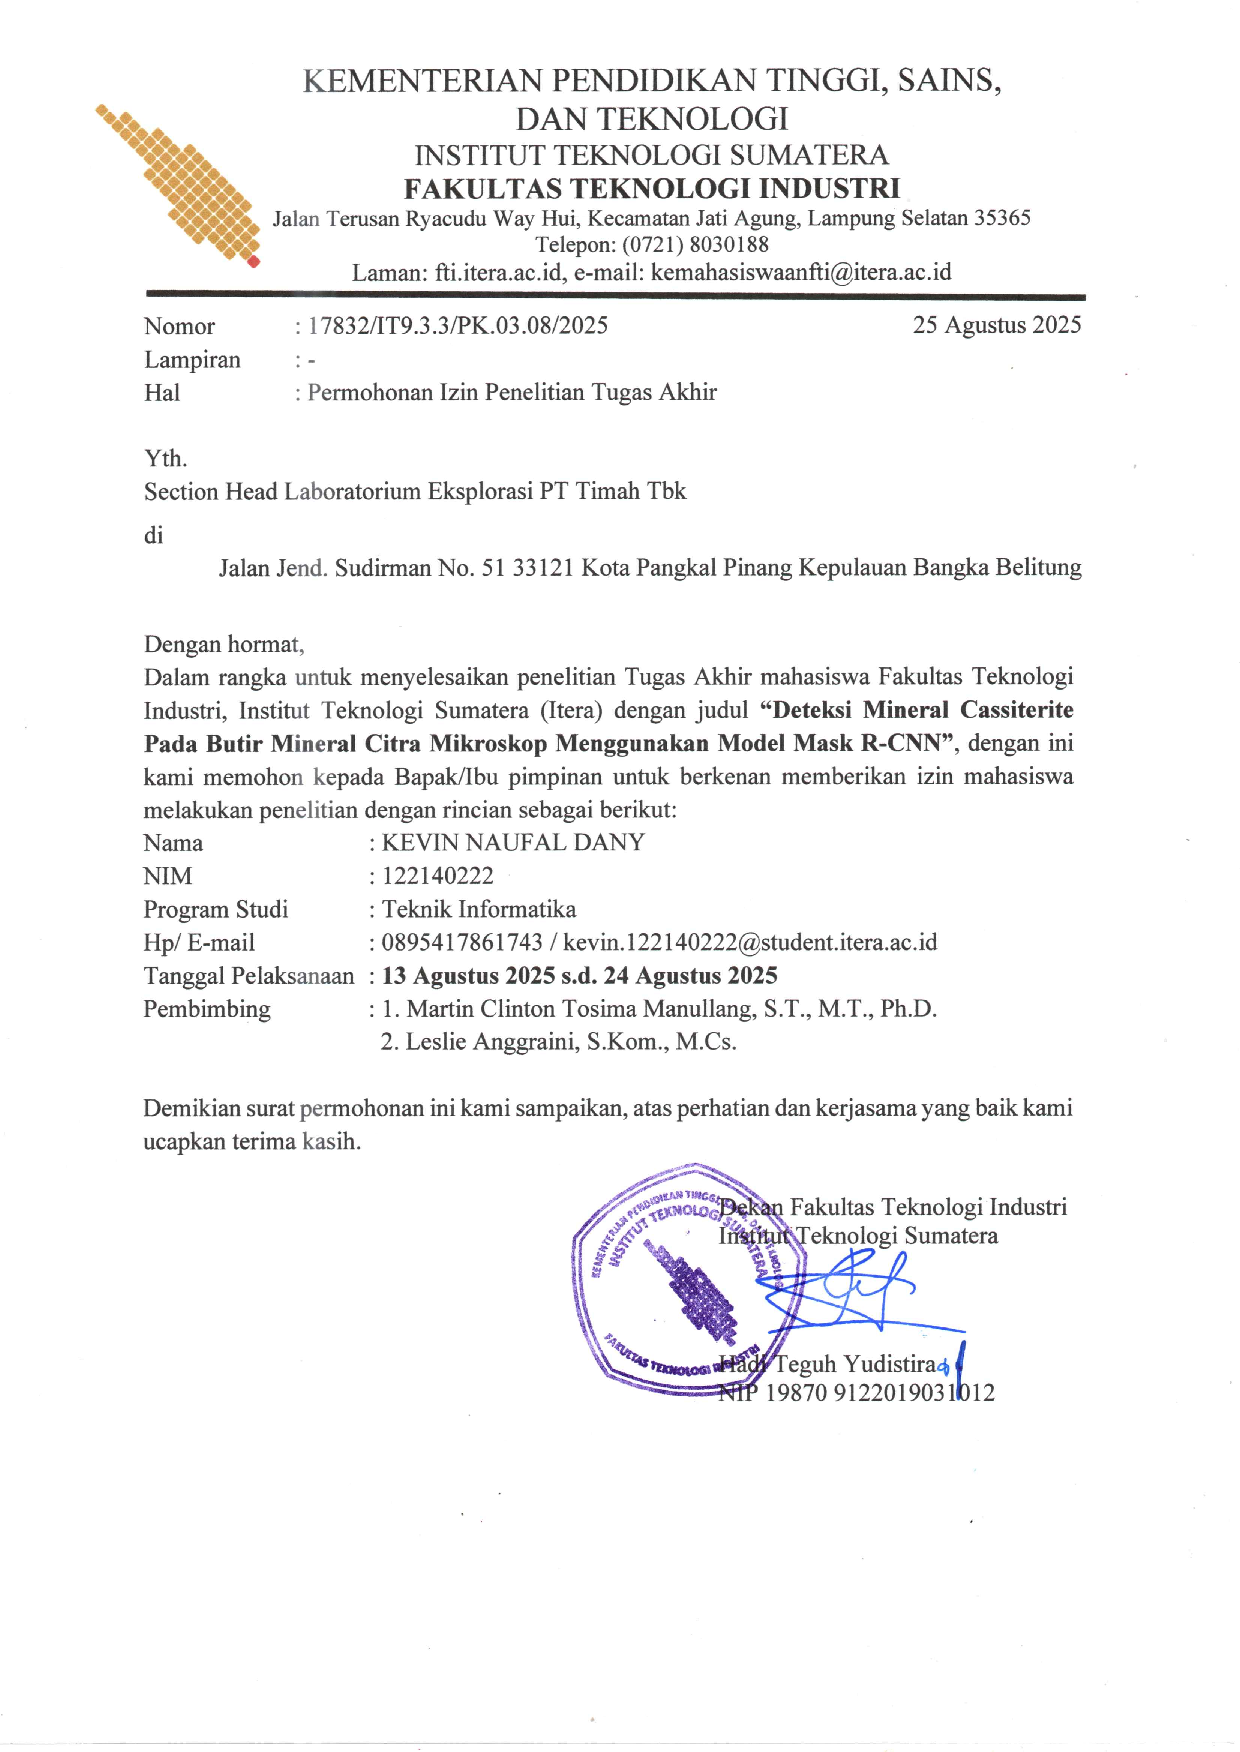
\includegraphics[page=1, width=0.85\textwidth]{doc/surat_izin_penelitian_kevin_pt_timah.pdf}
    \caption{Surat Izin Penelitian Tugas Akhir ke Laboratorium Eksplorasi PT Timah Tbk}
    \label{fig:SuratIzinPenelitian}
\end{figure}

\begin{figure}[H] % Kalau menggunakan H, posisi gambar akan tepat dibawah teks
    \centering
    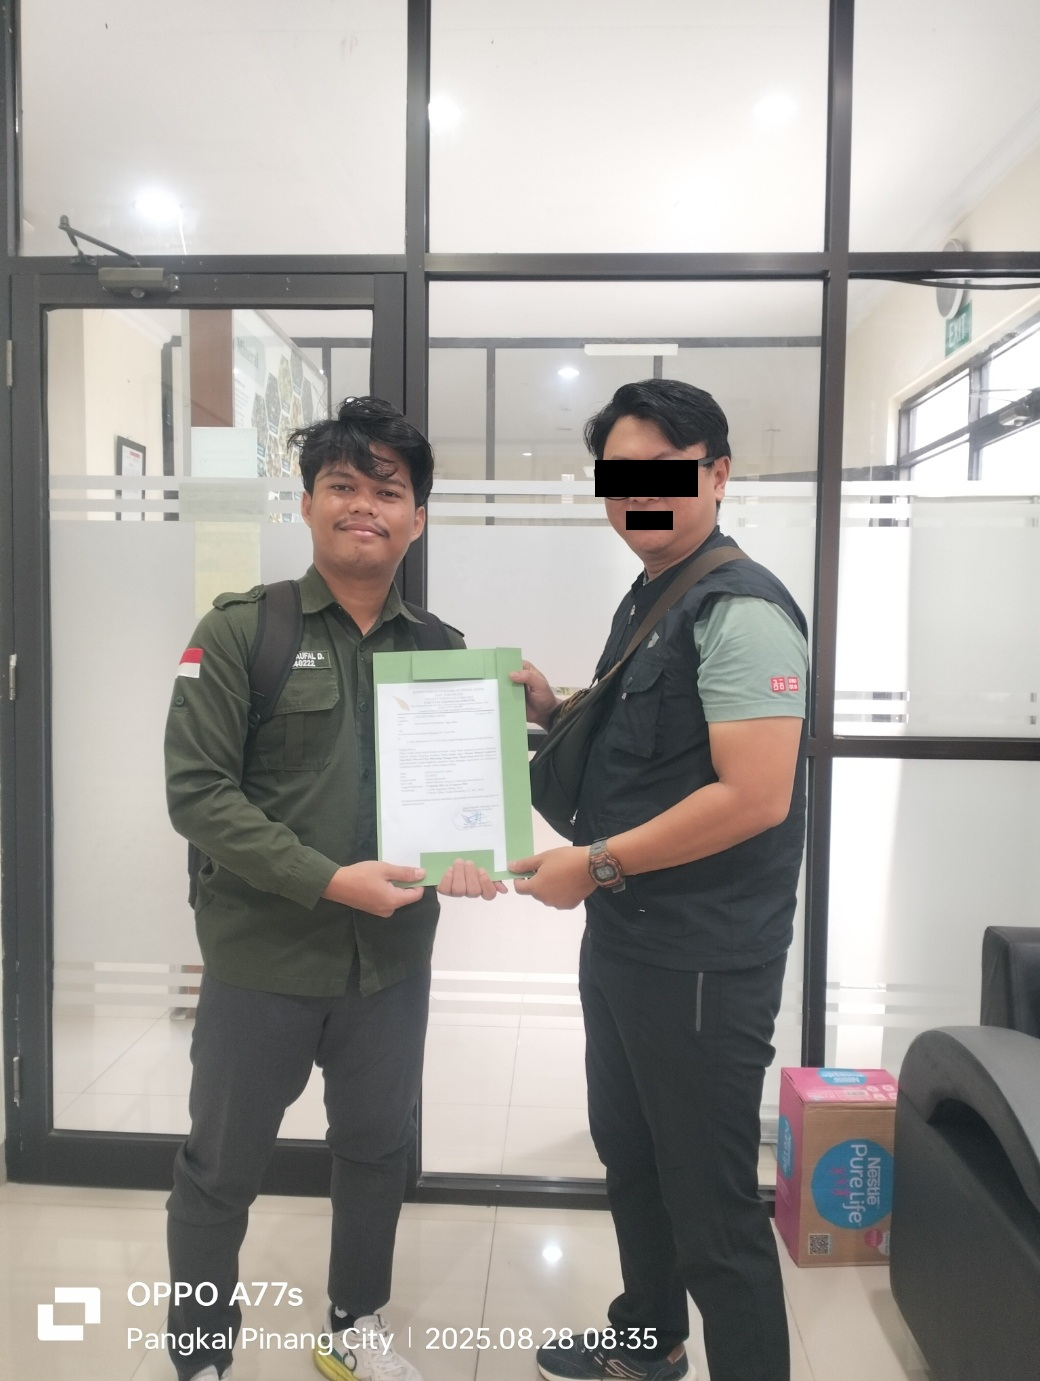
\includegraphics[width=0.85\textwidth]{figure/lampiran/pakMesaSurat.jpg}
    \caption{Surat Pengantar Penelitian}
    \label{fig:PengantarPenelitian}
\end{figure}

\section{Lampiran 2. Dataset} \label{lampiran:Dataset}

\begin{figure}[H] % Kalau menggunakan H, posisi gambar akan tepat dibawah teks
    \centering
    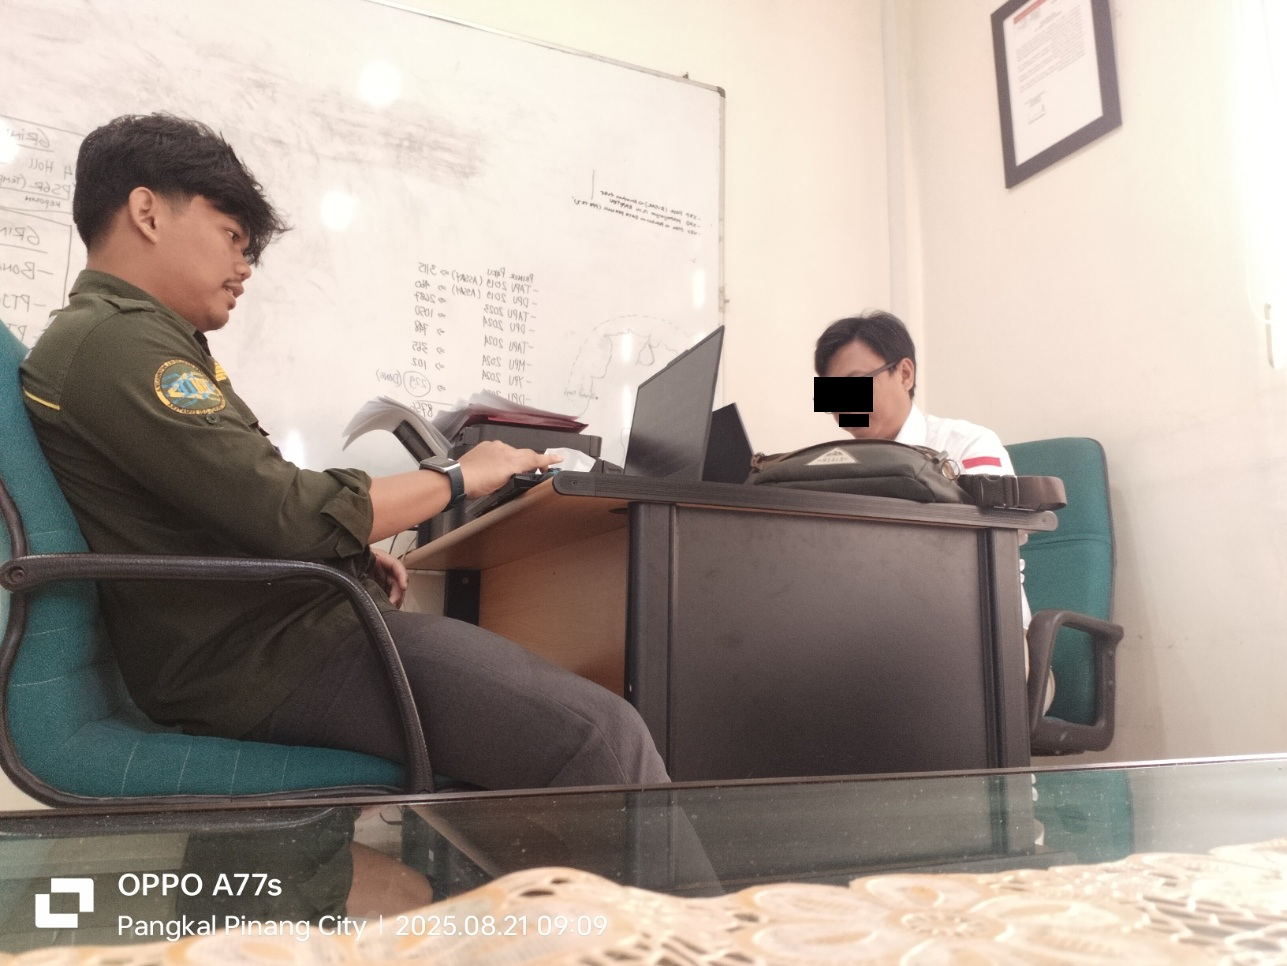
\includegraphics[width=0.85\textwidth]{figure/lampiran/pakMesaData.jpg}
    \caption{Pengumpulan Data}
    \label{fig:PengumpulanData}
\end{figure}


\section{Lampiran 3. Hasil Wawancara} \label{lampiran:Wawancara}
\begin{figure}[H] % Kalau menggunakan H, posisi gambar akan tepat dibawah teks
    \centering
    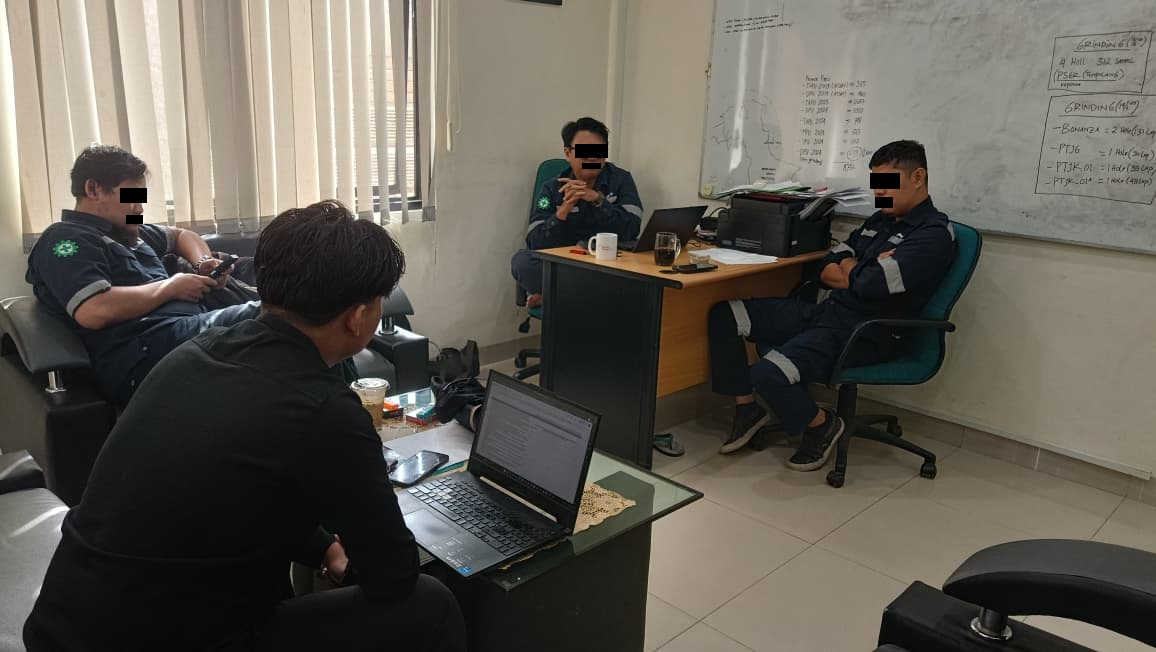
\includegraphics[width=0.85\textwidth]{figure/lampiran/fotoWwc.jpg}
    \caption{Wawancara dengan Bapak Mesa Madestriasa}
    \label{fig:Wawancara}
\end{figure}

{\footnotesize
\begin{longtable}{|p{0.025\textwidth}|p{0.45\textwidth}|p{0.45\textwidth}|}
\caption{List Pertanyaan dan Jawaban dari Hasil Wawancara}
\label{table:wawancara-bijih-timah} \\
\hline
\centering\textbf{No} & \centering\textbf{Pertanyaan} & \centering\arraybackslash\textbf{Jawaban} \\
\hline
\endfirsthead

\hline
\centering\textbf{No} & \centering\textbf{Pertanyaan} & \centering\arraybackslash\textbf{Jawaban} \\
\hline
\endhead

1 &
Di sini saya sedang melakukan penelitian mengenai deteksi bijih timah pada citra microskop menggunakan kecerdasan buatan gitu pak, jadi kasarnya itu membuat suatu program gitu yang dapat mendeteksi dan memprediksi ada berapa dan dimana saja si bijih timah pada suatu citra atau foto microskop tersebut seperti menggunakan Microscope Software, menurut apakah apakah penelitian ini bisa di implementasikan dan apakah menurut bapak ini dapat di implementasikan dalam analisis laboratorium saat ini pak &
Bisa sekali dan sudah ada juga project di sebelum2 nya yang dimana sudah 2 tahun yang lalu juga untuk membuat ai tetapi masih sekitar 50\% akurasi prediksi nya, karena saat ini harus 3 kali bolak balik sampel untuk dalam 1 sampel dan pasti ada faktor subjektivitas, dengan ai bisa mengurangi itu \\
\hline

2 &
Apakah ada standar ukuran bijih timah dalam satuan mesh yang di gunakan untuk analisis labolatorium saat ini &
Standar ukuran kita pakai kalau GCA itu tiga mesh atau 3 fraksi 48, 100 -100 mesh \\
\hline

3 &
Apakah ada karakteristik utama dan standar tertentu biji timah (cassiterite) yang membedakan satu jenis sama jenis lain berdasarkan warna atau bentuk seperti (katalog atau ensiklopedia timah) gitu pak? &
Kalau warna timah itu macam-macam. Ada yang dari mulai coklat, hitam, terus ada merah pun ada. kilap minyak / kilap solar nya yang khusus yang ada di cassiterite, ukuran nya tu ronded sampai sub-ronded tidak ada yang angular tidak ad yang tajam2 gitu, karena suda di masukkan ke mesin lalu mineral akan menggerus dirinya sendiri hingga berukuran ronded sampai sub-ronded, katalog ada tetapi seperti poster hanya seperti buku mengenai macam2 mineral'' \\
\hline

4 &
Apa saja jenis biji timah yang paling sering muncul di sampel bapak, dan apa ciri-cirinya yang dapat di lihat dari segi visual terutama foto? &
Jelas bisa, masing2 daerah mempunyai karakteristik bijih timah nya tersendiri jadi yang sering muncul ya seperti pada sebelumnya. Warnanya ya hitam, warna coklat, Coklat gelap, merah gelap. Kilapnya, kilap minyak. Jadi sering muncul kayak lemak-lemak gitu kalau dimulai mikroskop. istilahnya kayak daging dan serat2 daging gitu \\
\hline

5 &
Dari pengalaman bapak, apa tantangan terbesar dalam mengidentifikasi biji timah secara manual di lab? &
Kalau yang masih baru atau masih belajar biasanya yang tertukar itu antara mineral cassiterite dan ilminite, di karenakan ilminite berwarna hitam dan berkilap karena kalau yang masih baru2 masih belum bisa membedakan kilapnya saja \\
\hline

6 &
Ada nggak pola khusus atau ciri-ciri yang biasanya bapak cari, buat klasifikasi biji timah? &
Kilap minyak itu lah karena kilap minyak di cassiterite sangat khas \\
\hline

7 &
Apakah ada jenis biji timah tertentu yang sering bikin bingung waktu dianalisis pak seperti nemuin yang warnanya mirip banget dengan mineral lain atau memang di modifikasi untuk bijih timah nya (di pilok atau di kasih kecap gitu), seberapa sering di temukan dan gimana cara mengatasinya &
Di karenakan sudah melalui beberapa proses seperti cuci di keringkan sampel itu sebelumnya, sebelum menjadi sebuah sample sebelum di lakukan tim analisis jadi tetep ketahuan walau di pilok pun tetap ketahuan karena kilap minyak cassiterite itu \\
\hline

8 &
Bagaimana proses bapak nyiapin sampel sebelum difoto di mikroskop? &
Untuk penyiapan sampel itu sampel sudah datang clean ke lab karena sudah di keringin jadi langsung di analisa saja, kecuali kalo sampel kasar kita masukkan ke oven atau di goreng dulu jika sudah baru masuk ke lab \\
\hline

9 &
Ada nggak faktor di lab, kayak pencahayaan atau pengaturan mikroskop, yang bisa pengaruhi warna atau tampilan biji timah di foto? &
Sangat berpengaruh, karena data yang saya terima itu juga masih beragam pencahayaannya dan bagusnya itu di dalam 1 mikroskop dan dalam satu ruangan studio jadi pencahayaannya jadi seragam, tpi kalo untuk visual biasa tidak terlalu berpengaruh sekali \\
\hline

10 &
Software apa yang bapak pakai buat motret biji timah di mikroskop? lalu apakah ada format khusus buat gambarnya (.jpg/ .png)? &
Outputnya jpg \\
\hline

11 &
Apakah ukuran 48, 100, -100 Mesh ini punya perbedaan signifikan di lab, misalnya dalam cara pemrosesan atau analisis? &
Ada paling kayak 48 itu kasar, 100 itu sedang lah, -100 halus, kalo semakin kecil semakin membulat, dan misal dia berbeda mesh dalam 1 sampel itu kadang setiap mineral itu menimpa gitu saling menimpa mineral lain \\
\hline

12 &
Kalau saya ingin membuat suatu kecerdasan buatan yang bener-bener akurat, data apa yang menurut bapak wajib banget ada di dataset? &
Dari saya si maunya kasarnya dulu saja untuk menentukan persentase kasiterite nya dulu saja, apakah ai itu bisa atau tidak menemukan mineral kassiterit, jikalau sudah bisa ini sudah good untuk ai nya, persentase yang di maksud itu mengabaikan mineral selain kasiterit seperti semisal ada 100 butir dalam 1 sampel ternyata ada 60 mineral kasiterit berarti itu 60\% gitu untuk mahasiswa seperti itu aja \\
\hline

13 &
Berapa jumlah minimal gambar yang bapak saranin buat dataset biar hasil kecerdasan buatan akurat? &
Untuk data saat ini ada 1046 jadi seharusnya cukup untuk ai ya \\
\hline

\end{longtable}
}


\section{Lampiran 4. Observasi} \label{lampiran:Observasi}
\begin{figure}[H]
    \centering
    % ===== Baris atas =====
    \begin{subfigure}[t]{0.48\textwidth}
        \centering
        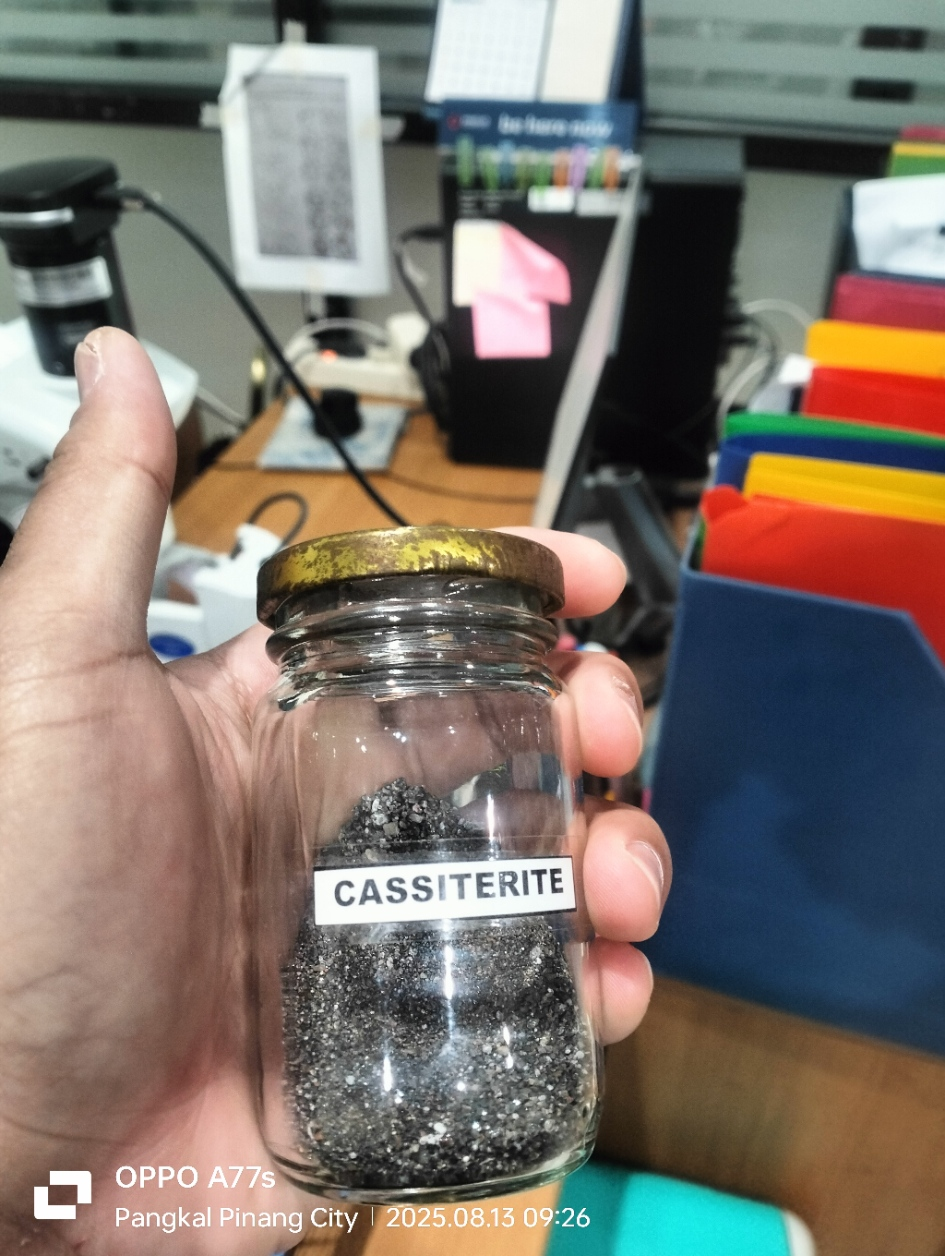
\includegraphics[width=\textwidth]{figure/lampiran/contohMineralCass.jpg}
        \caption{Contoh Mineral Cassiterite}
        \label{fig:ContohMineralCassiterite}
    \end{subfigure}
    \hfill
    \begin{subfigure}[t]{0.48\textwidth}
        \centering
        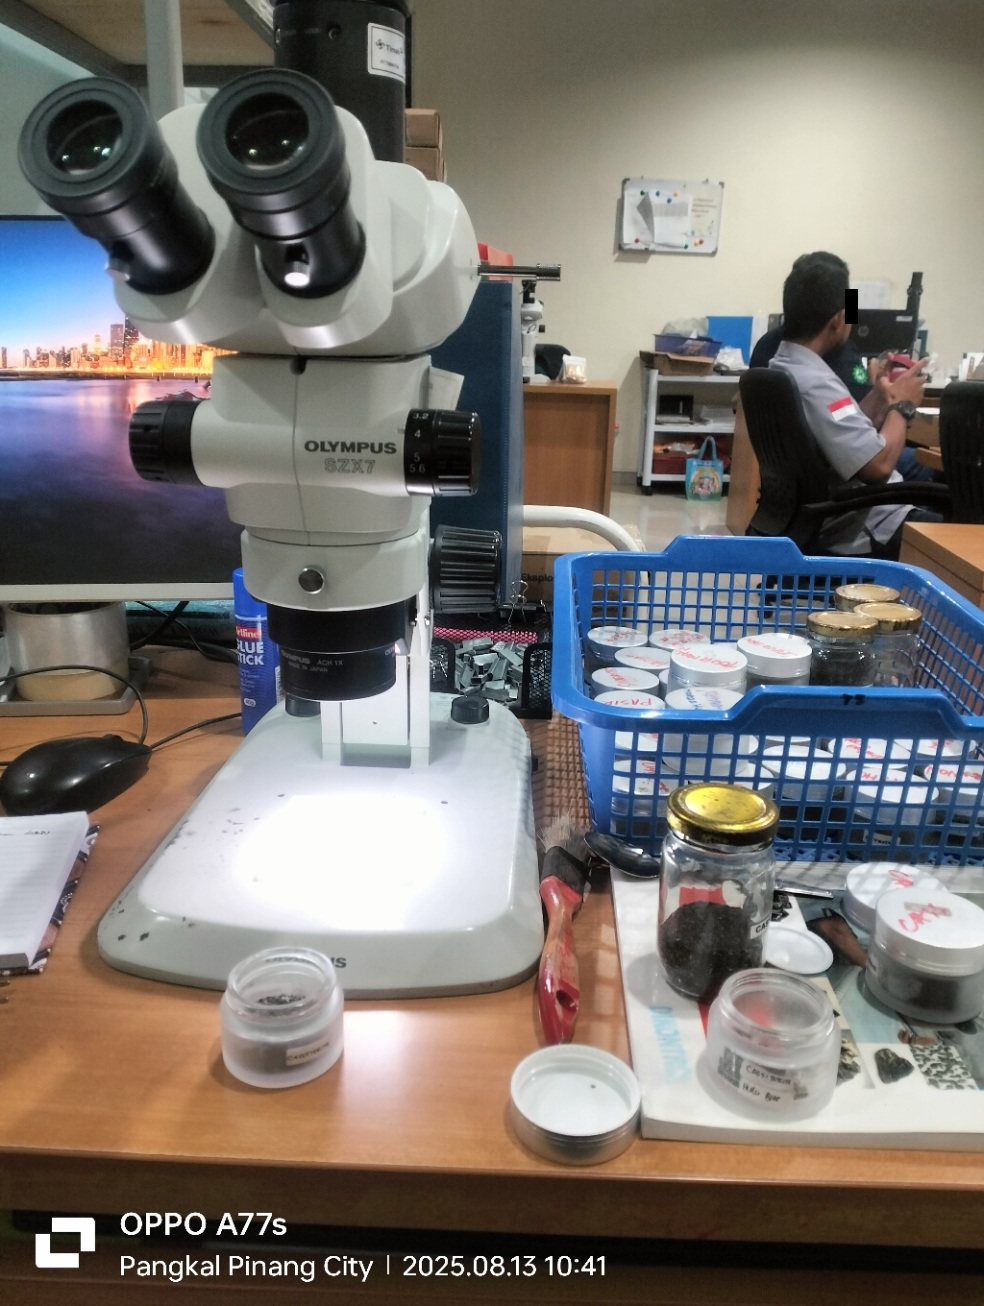
\includegraphics[width=\textwidth]{figure/lampiran/contohMikroskop.jpg}
        \caption{Contoh Mikroskop Trinokuler}
        \label{fig:ContohMikroskopTrinokuler}
    \end{subfigure}

    \vspace{0.4cm}

    % ===== Baris bawah =====
    \begin{subfigure}{0.7\textwidth}
        \centering
        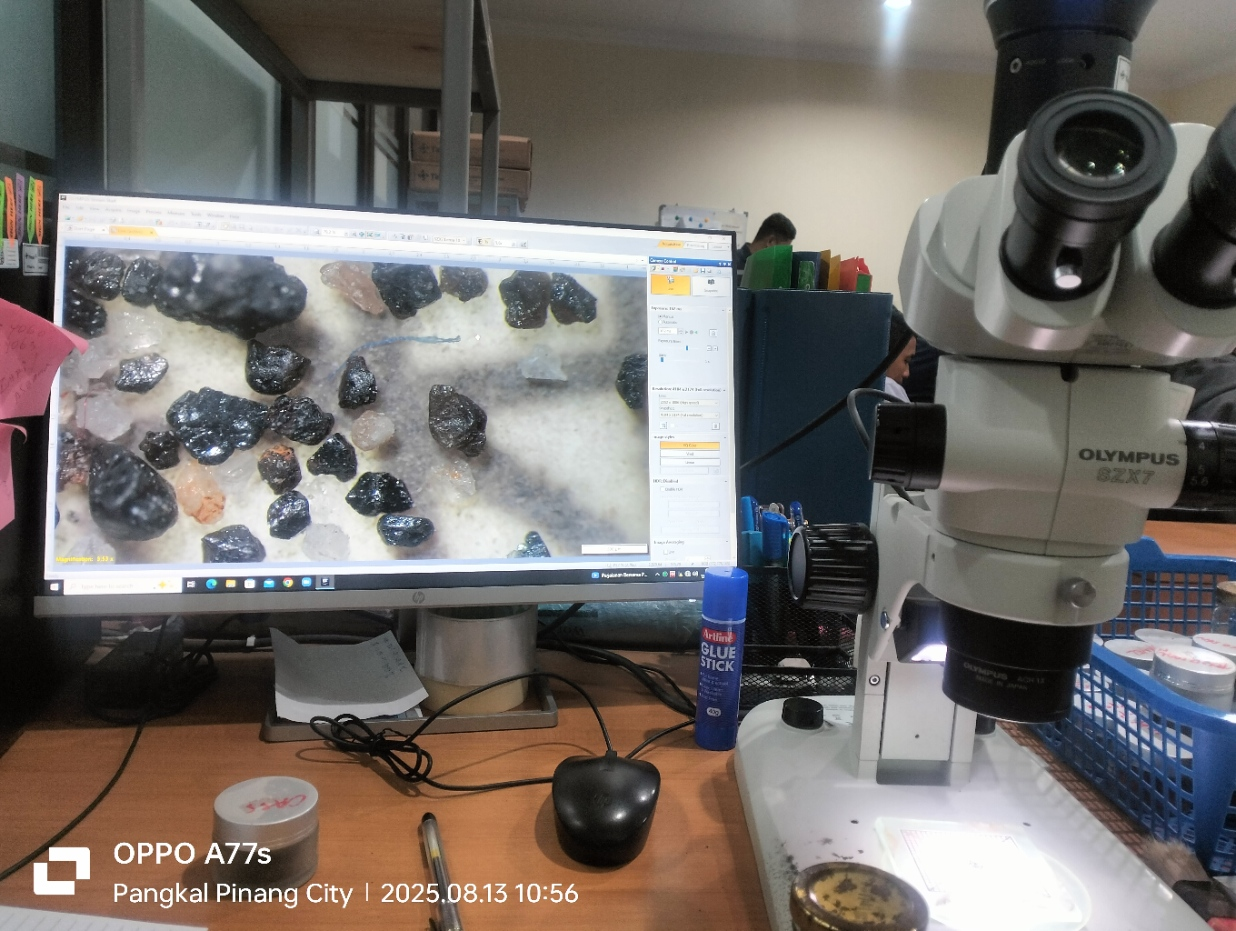
\includegraphics[width=\textwidth]{figure/lampiran/contohHasilCitraMikroskop.jpg}
        \caption{Contoh Hasil Citra Mikroskop}
        \label{fig:ContohHasilCitraMikroskop}
    \end{subfigure}

    \caption{Contoh Mineral Kasiterit, Mikroskop Trinokuler, dan Hasil Citra Mikroskop}
    \label{fig:ContohGabunganMikroskop}
\end{figure}


\begin{figure}[H]
    \centering
    % ===== Baris atas =====
    \begin{subfigure}[t]{0.48\textwidth}
        \centering
        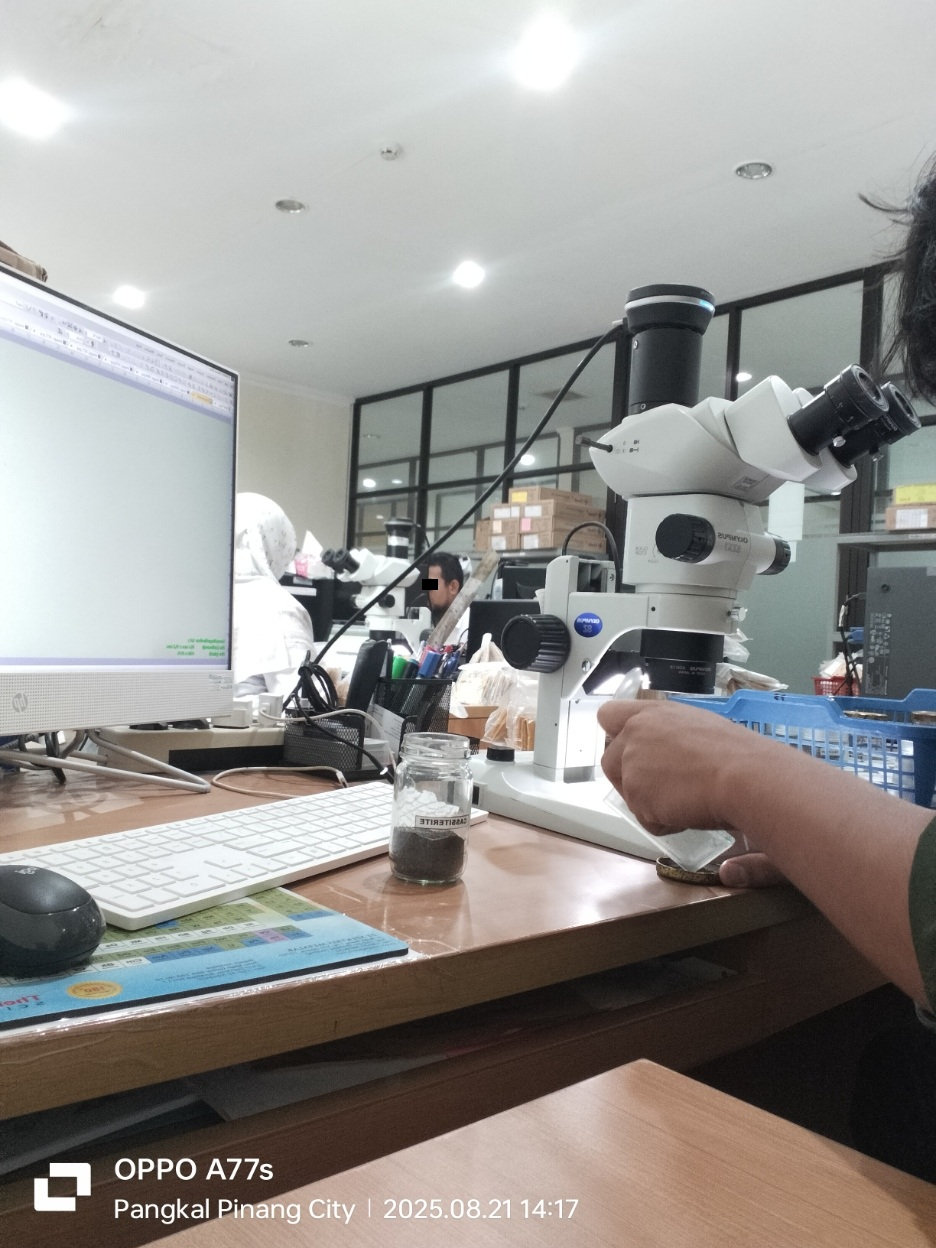
\includegraphics[width=\textwidth]{figure/lampiran/penampangMineral.jpg}
        \caption{Membersihkan Penampang Mineral}
        \label{fig:MembersihkanPenampangMineral}
    \end{subfigure}
    \hfill
    \begin{subfigure}[t]{0.48\textwidth}
        \centering
        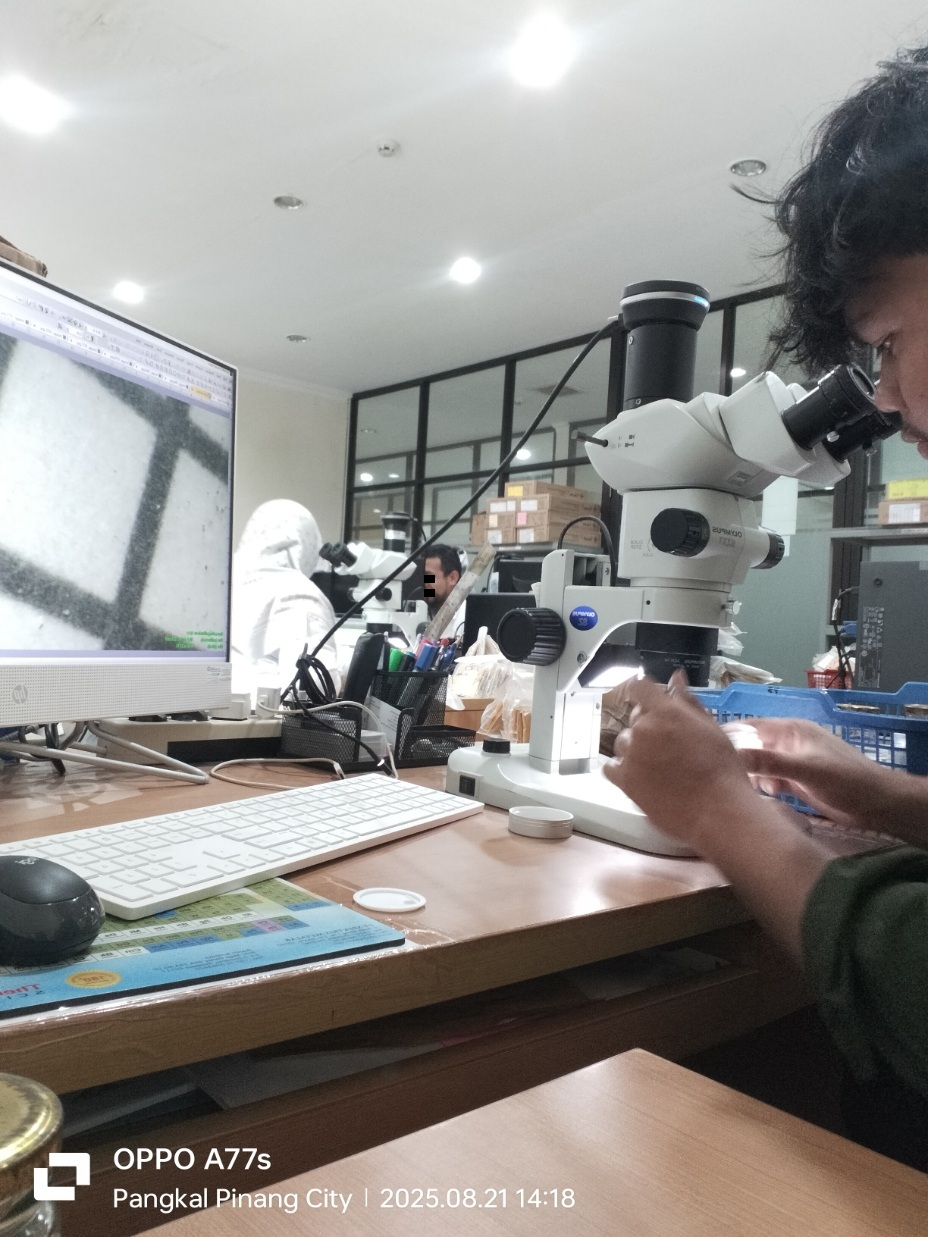
\includegraphics[width=\textwidth]{figure/lampiran/mencobaMenaburiMineralDiPenampang.jpg}
        \caption{Menaburi Mineral Kasiterit di Penampang Mineral}
        \label{fig:MenaburiMineralKasiteritDiPenampang}
    \end{subfigure}

    \vspace{0.4cm}

    % ===== Baris bawah =====
    \begin{subfigure}{0.6\textwidth}
        \centering
        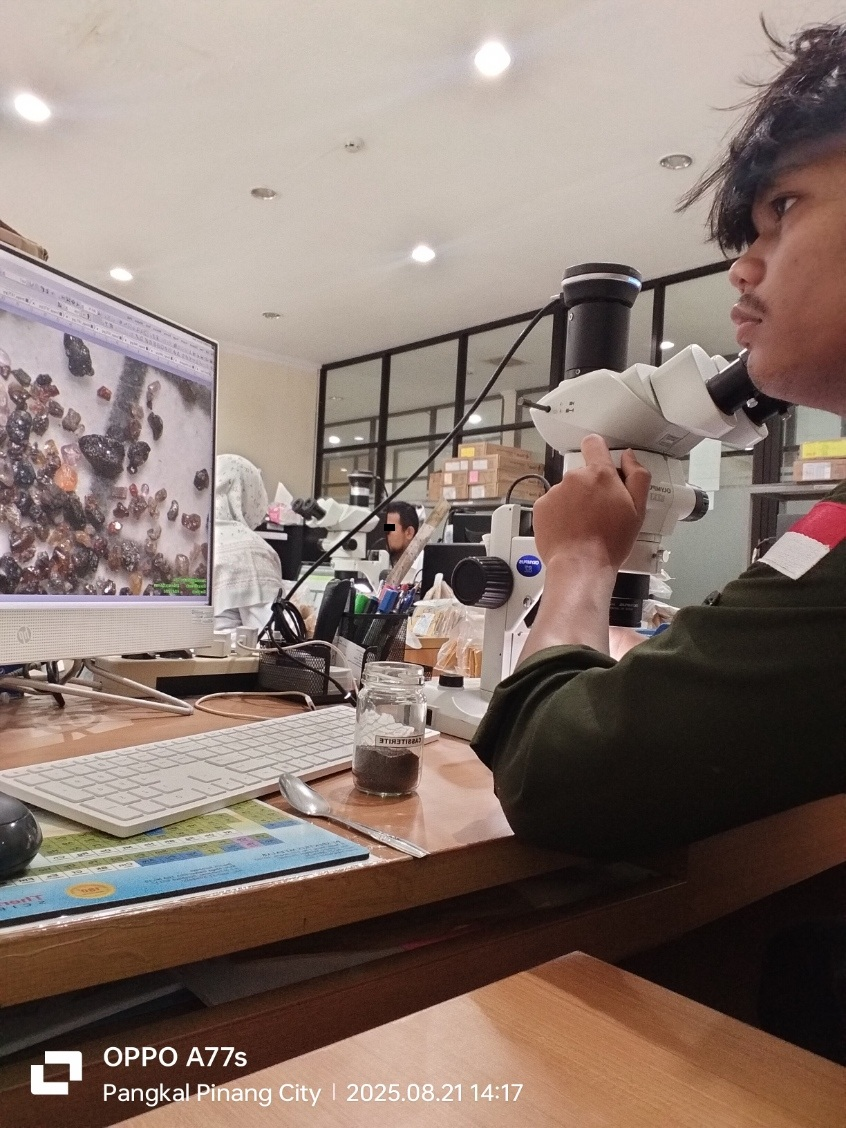
\includegraphics[width=\textwidth]{figure/lampiran/mencobaMikroskop.jpg}
        \caption{Melakukan Pengamatan Terhadap Citra Butiran Mineral Kasiterit dan Mineral Ikutan Lainnya untuk Memahami Karakteristik Secara Visual Menggunakan Mikroskop Trinokuler}
        \label{fig:MenggunakanMikroskopTrinokuler}
    \end{subfigure}

    \caption{Tahapan Persiapan dan Pengamatan Mineral Kasiterit Menggunakan Mikroskop Trinokuler}
    \label{fig:ProsesPengamatanMineralKasiterit}
\end{figure}


\section{Lampiran 5. Hasil Evaluasi Model} \label{lampiran:HasilEvaluasiModel}
\subsection*{Variasi 1 \textit{Mask} R-CNN ResNet50 FPN V1 + \textit{Amodal} + SGD}
\begin{figure}[H]
    \centering
    \fbox{\begin{minipage}{0.95\textwidth}
        \centering
        \begin{tabular}{cc}
            
\includegraphics[width=0.45\textwidth]{figure/lampiran/lampiran_eval/resnet50_fpn_v1_amodal_sgd_lr0.01/fold1/loss_fold1.png} &
            
\includegraphics[width=0.45\textwidth]{figure/lampiran/lampiran_eval/resnet50_fpn_v1_amodal_sgd_lr0.01/fold1/mean_metrics_comparison_fold1.png} \\[0.5em]
            
\includegraphics[width=0.45\textwidth]{figure/lampiran/lampiran_eval/resnet50_fpn_v1_amodal_sgd_lr0.01/fold2/loss_fold2.png} &
            
\includegraphics[width=0.45\textwidth]{figure/lampiran/lampiran_eval/resnet50_fpn_v1_amodal_sgd_lr0.01/fold2/mean_metrics_comparison_fold2.png} \\[0.5em]
            
\includegraphics[width=0.45\textwidth]{figure/lampiran/lampiran_eval/resnet50_fpn_v1_amodal_sgd_lr0.01/fold3/loss_fold3.png} &
            
\includegraphics[width=0.45\textwidth]{figure/lampiran/lampiran_eval/resnet50_fpn_v1_amodal_sgd_lr0.01/fold3/mean_metrics_comparison_fold3.png} \\[0.5em]
            
\includegraphics[width=0.45\textwidth]{figure/lampiran/lampiran_eval/resnet50_fpn_v1_amodal_sgd_lr0.01/fold4/loss_fold4.png} &
            
\includegraphics[width=0.45\textwidth]{figure/lampiran/lampiran_eval/resnet50_fpn_v1_amodal_sgd_lr0.01/fold4/mean_metrics_comparison_fold4.png} \\[0.5em]
            
\includegraphics[width=0.45\textwidth]{figure/lampiran/lampiran_eval/resnet50_fpn_v1_amodal_sgd_lr0.01/fold5/loss_fold5.png} &
            
\includegraphics[width=0.45\textwidth]{figure/lampiran/lampiran_eval/resnet50_fpn_v1_amodal_sgd_lr0.01/fold5/mean_metrics_comparison_fold5.png} \\
        \end{tabular}
    \end{minipage}}
    \caption{Hasil Evaluasi Model Variasi 1 \textit{Mask} R-CNN ResNet50 FPN V1 + \textit{Amodal} + SGD}
    \label{fig:HasilEvaluasiModel1}
\end{figure}

\subsection*{Variasi 2 \textit{Mask} R-CNN ResNet50 FPN V1 + \textit{Amodal} + Adam}
\begin{figure}[H]
    \centering
    \fbox{\begin{minipage}{0.95\textwidth}
        \centering
        \begin{tabular}{cc}
            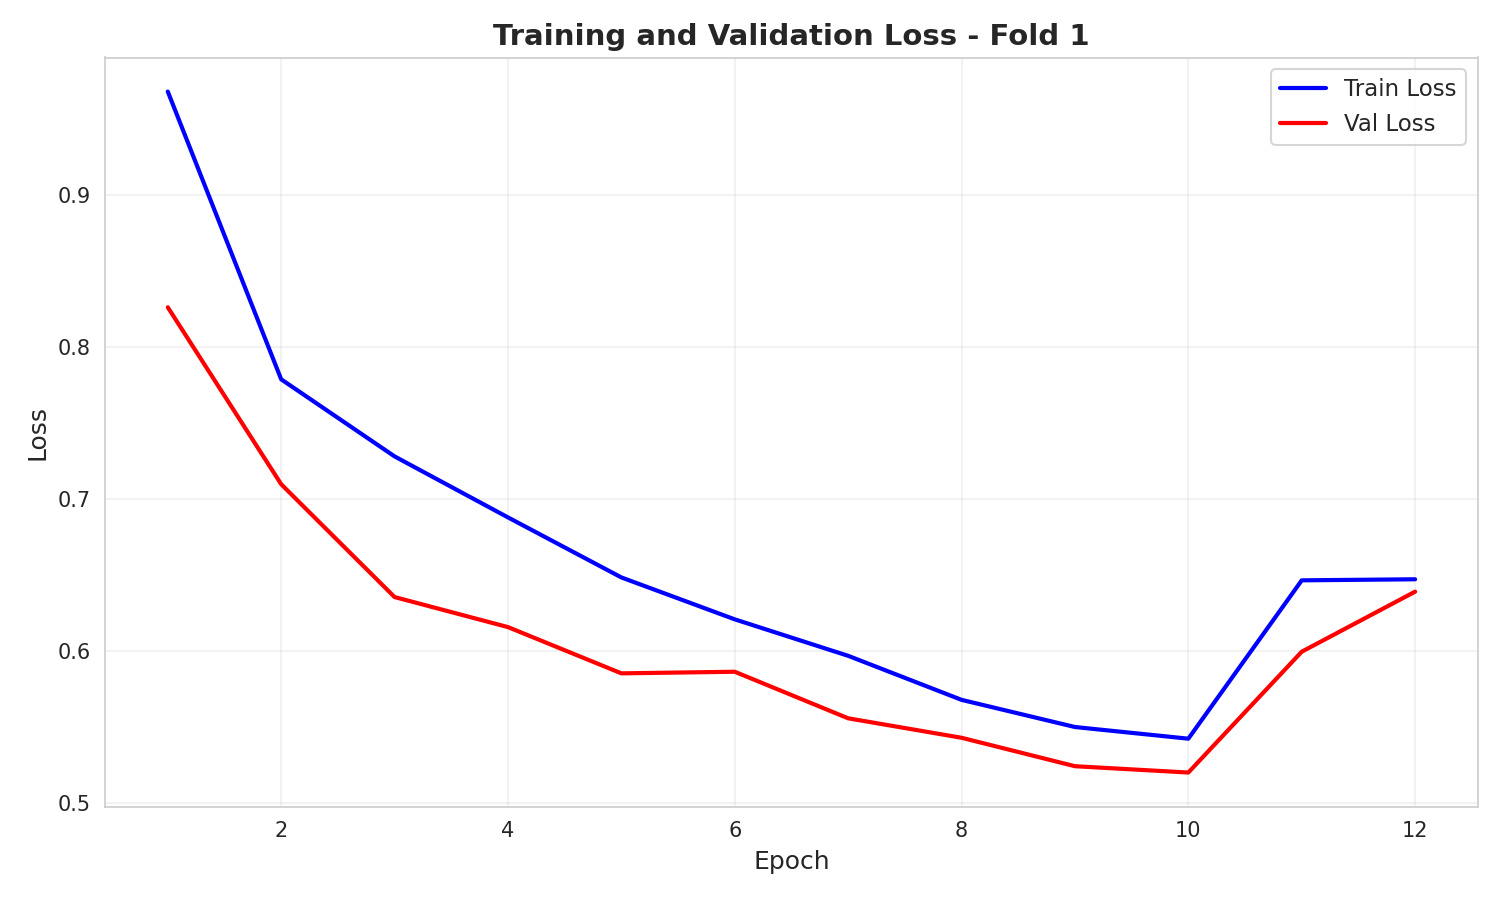
\includegraphics[width=0.45\textwidth]{figure/lampiran/lampiran_eval/resnet50_fpn_v1_amodal_adam_lr1e-04/fold1/loss_fold1.png} &
            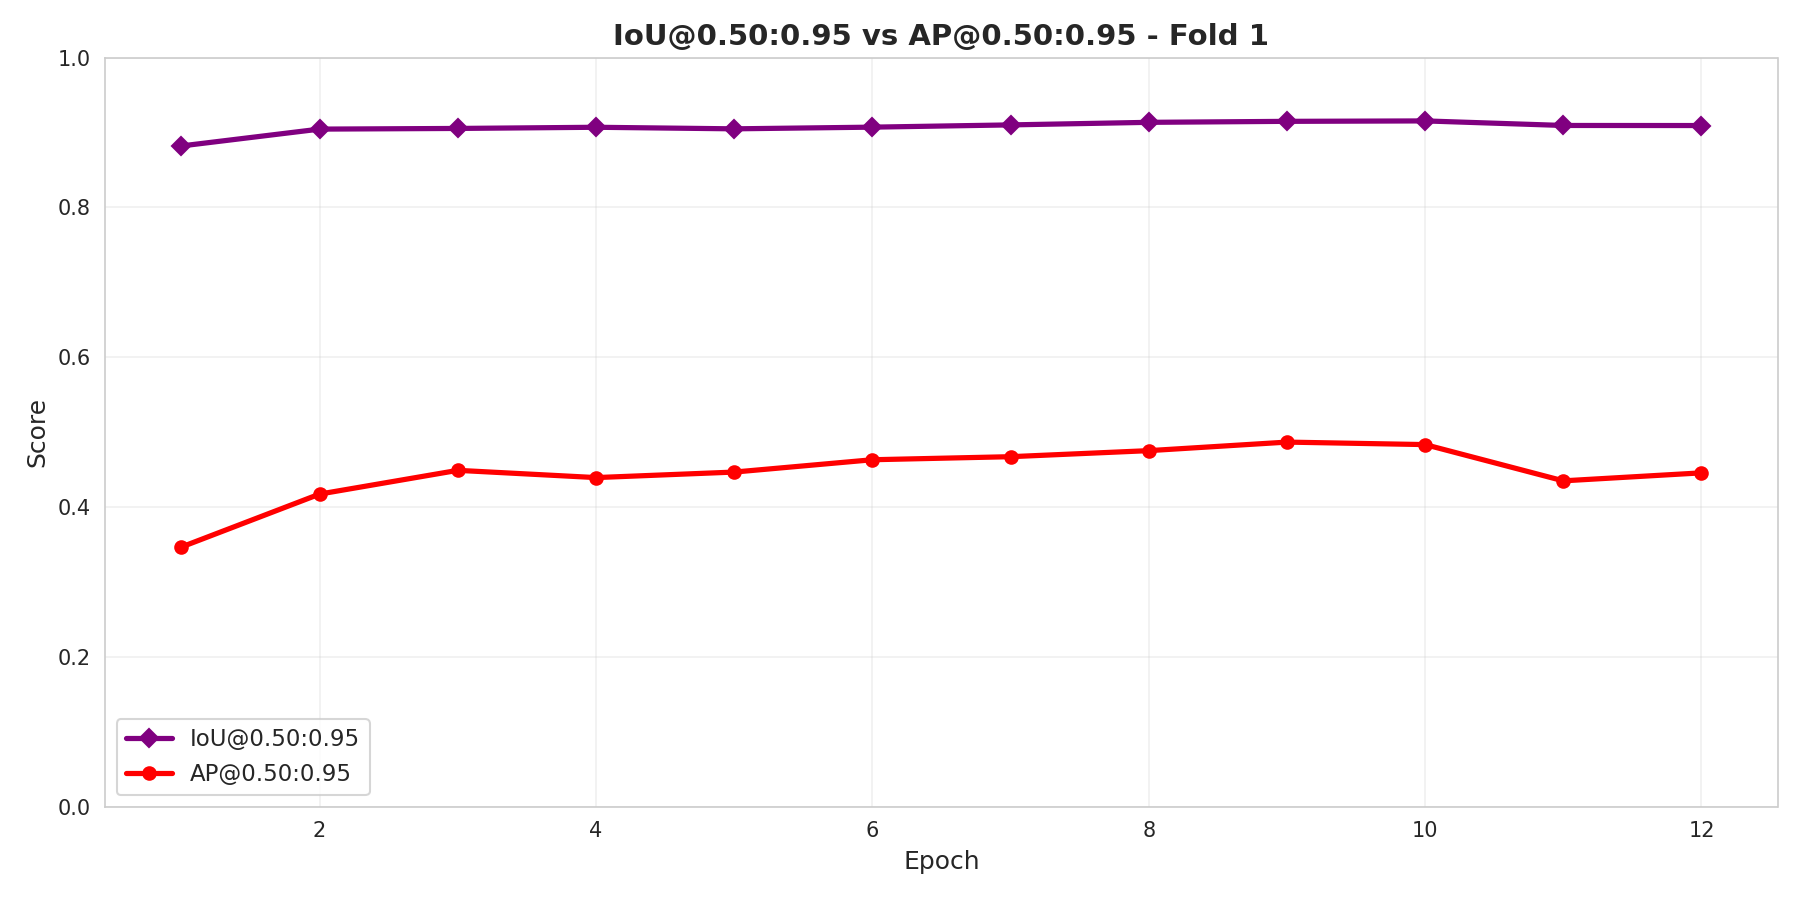
\includegraphics[width=0.45\textwidth]{figure/lampiran/lampiran_eval/resnet50_fpn_v1_amodal_adam_lr1e-04/fold1/mean_metrics_comparison_fold1.png} \\[0.5em]
            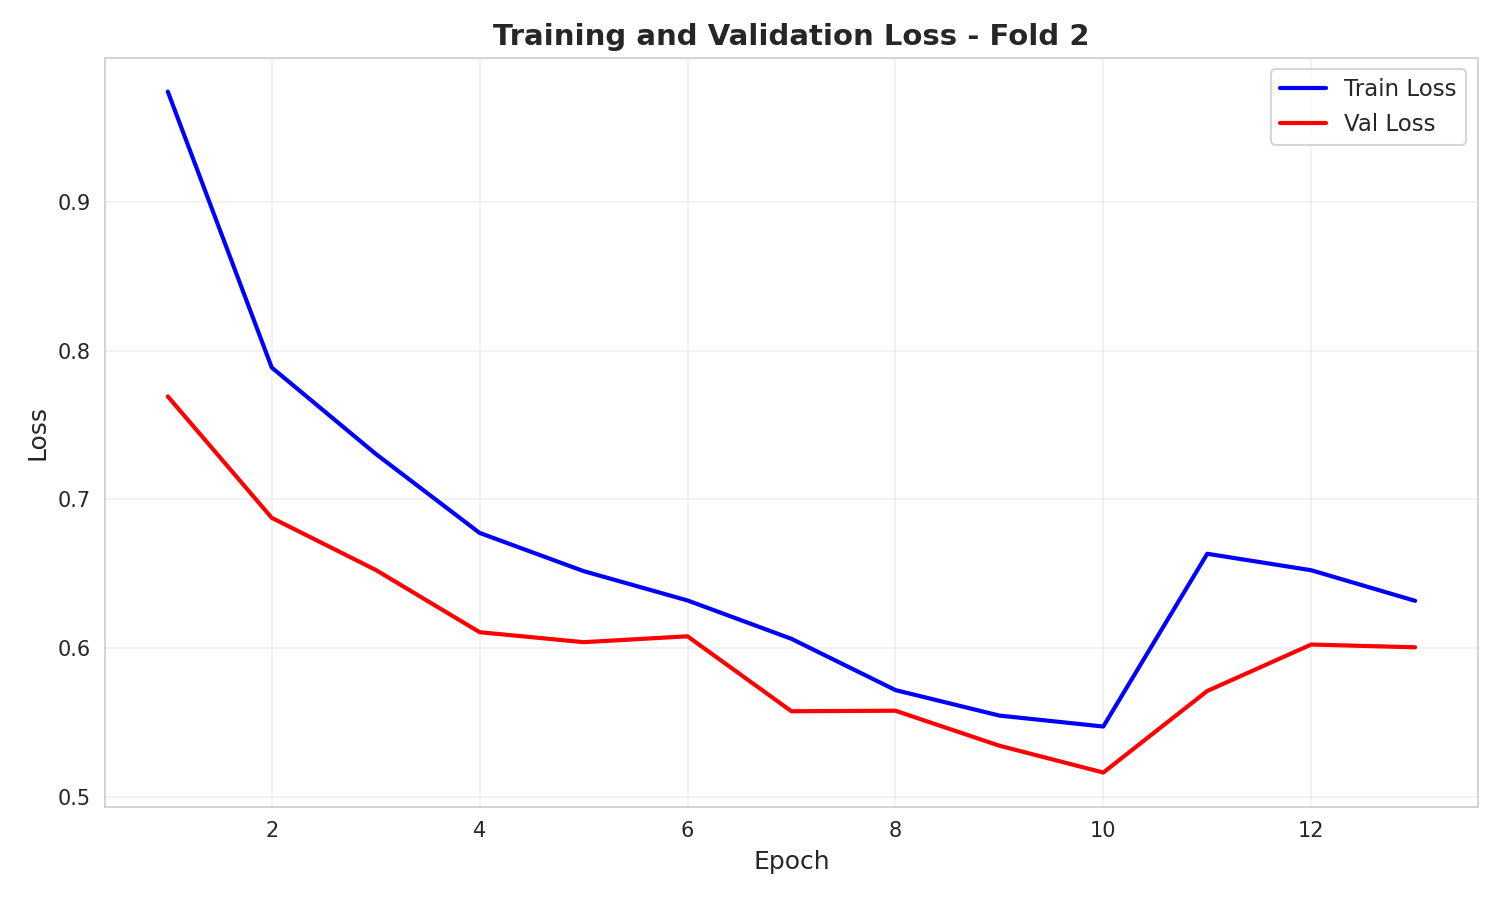
\includegraphics[width=0.45\textwidth]{figure/lampiran/lampiran_eval/resnet50_fpn_v1_amodal_adam_lr1e-04/fold2/loss_fold2.png} &
            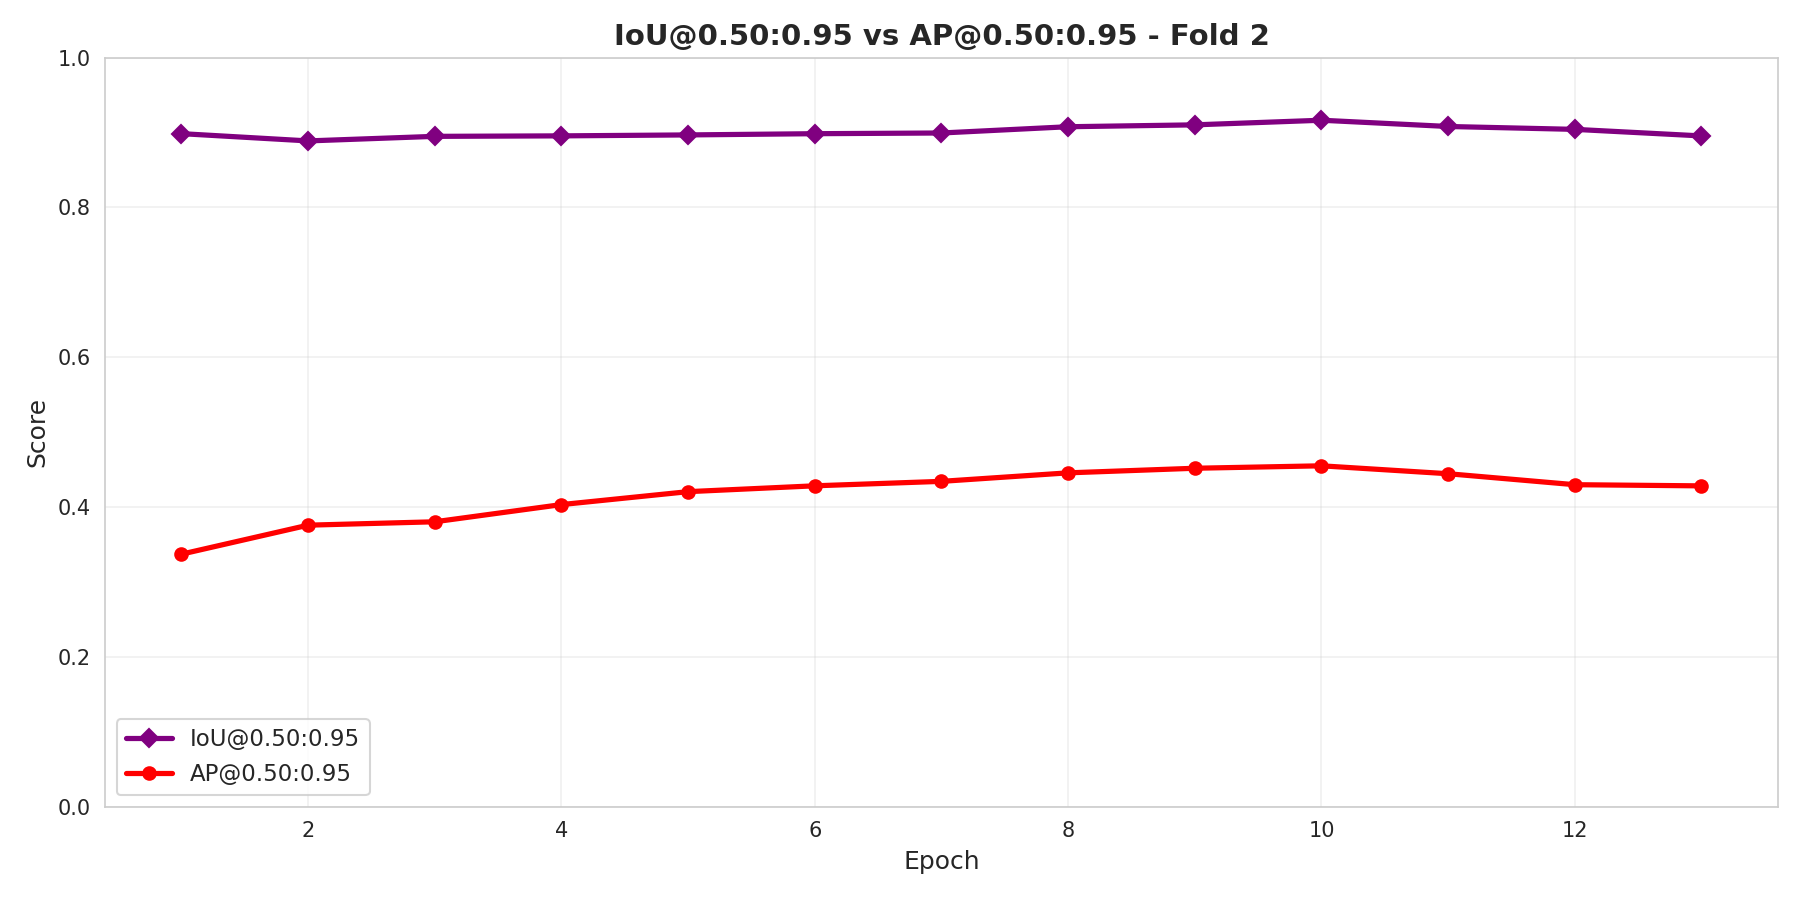
\includegraphics[width=0.45\textwidth]{figure/lampiran/lampiran_eval/resnet50_fpn_v1_amodal_adam_lr1e-04/fold2/mean_metrics_comparison_fold2.png} \\[0.5em]
            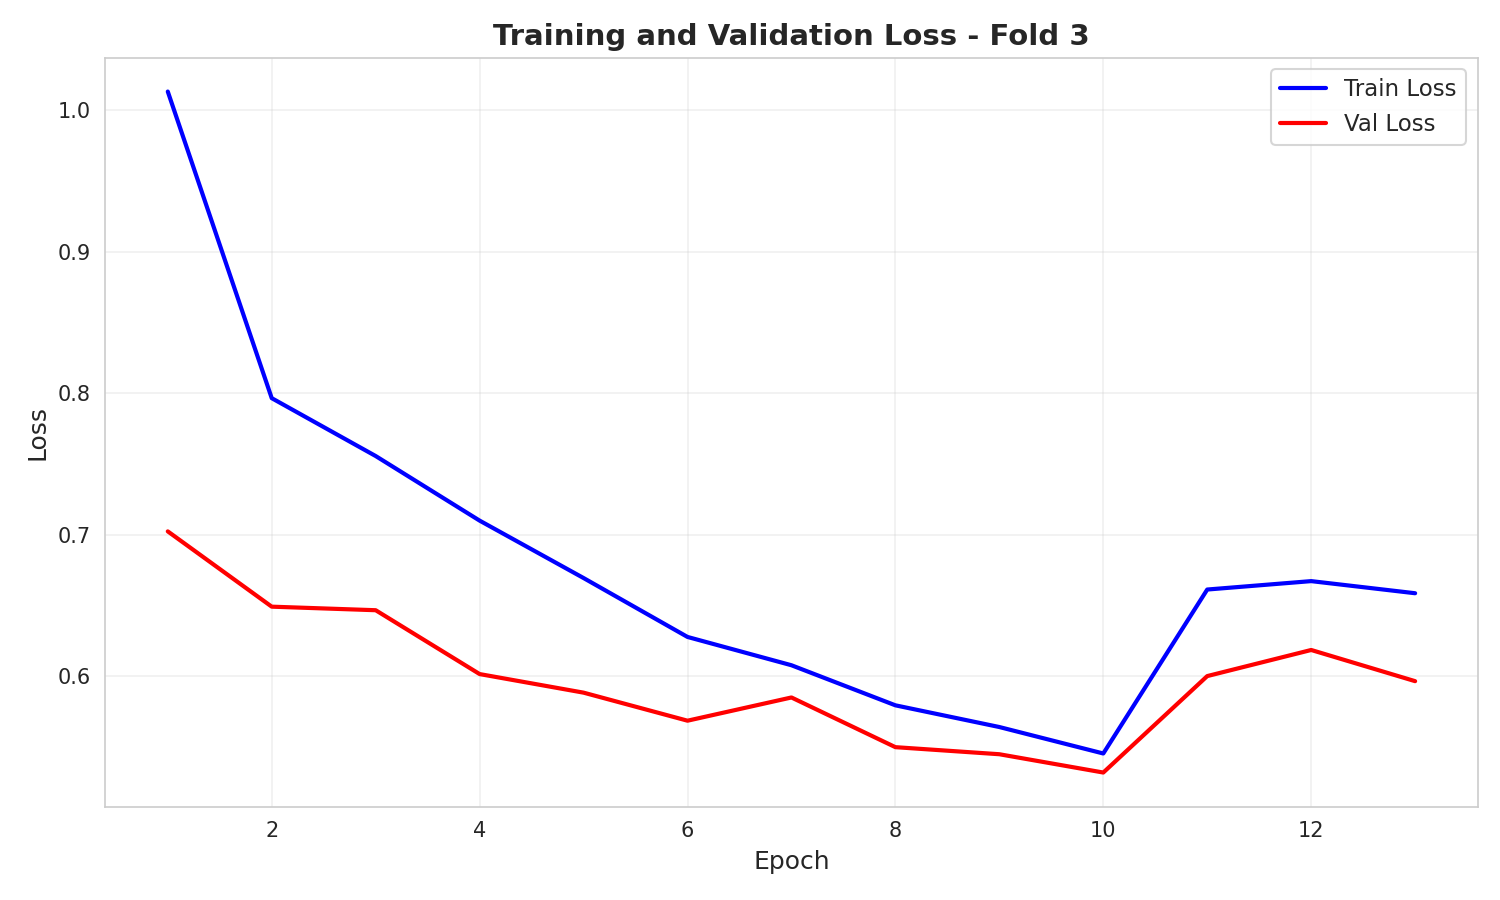
\includegraphics[width=0.45\textwidth]{figure/lampiran/lampiran_eval/resnet50_fpn_v1_amodal_adam_lr1e-04/fold3/loss_fold3.png} &
            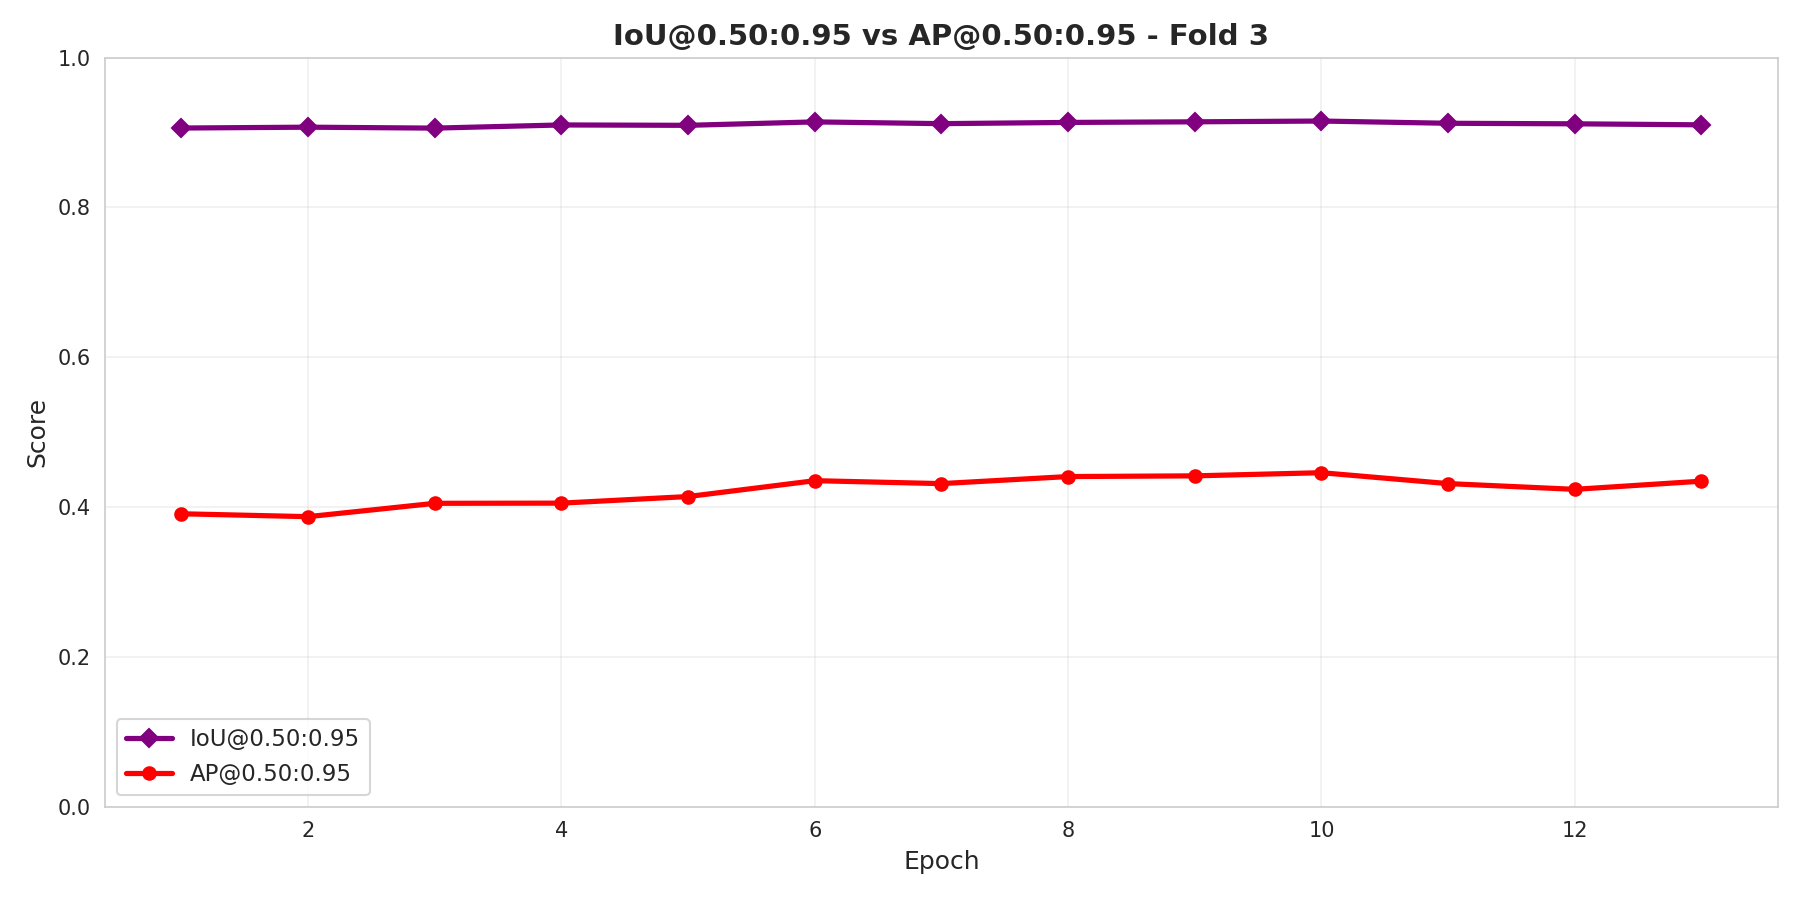
\includegraphics[width=0.45\textwidth]{figure/lampiran/lampiran_eval/resnet50_fpn_v1_amodal_adam_lr1e-04/fold3/mean_metrics_comparison_fold3.png} \\[0.5em]
            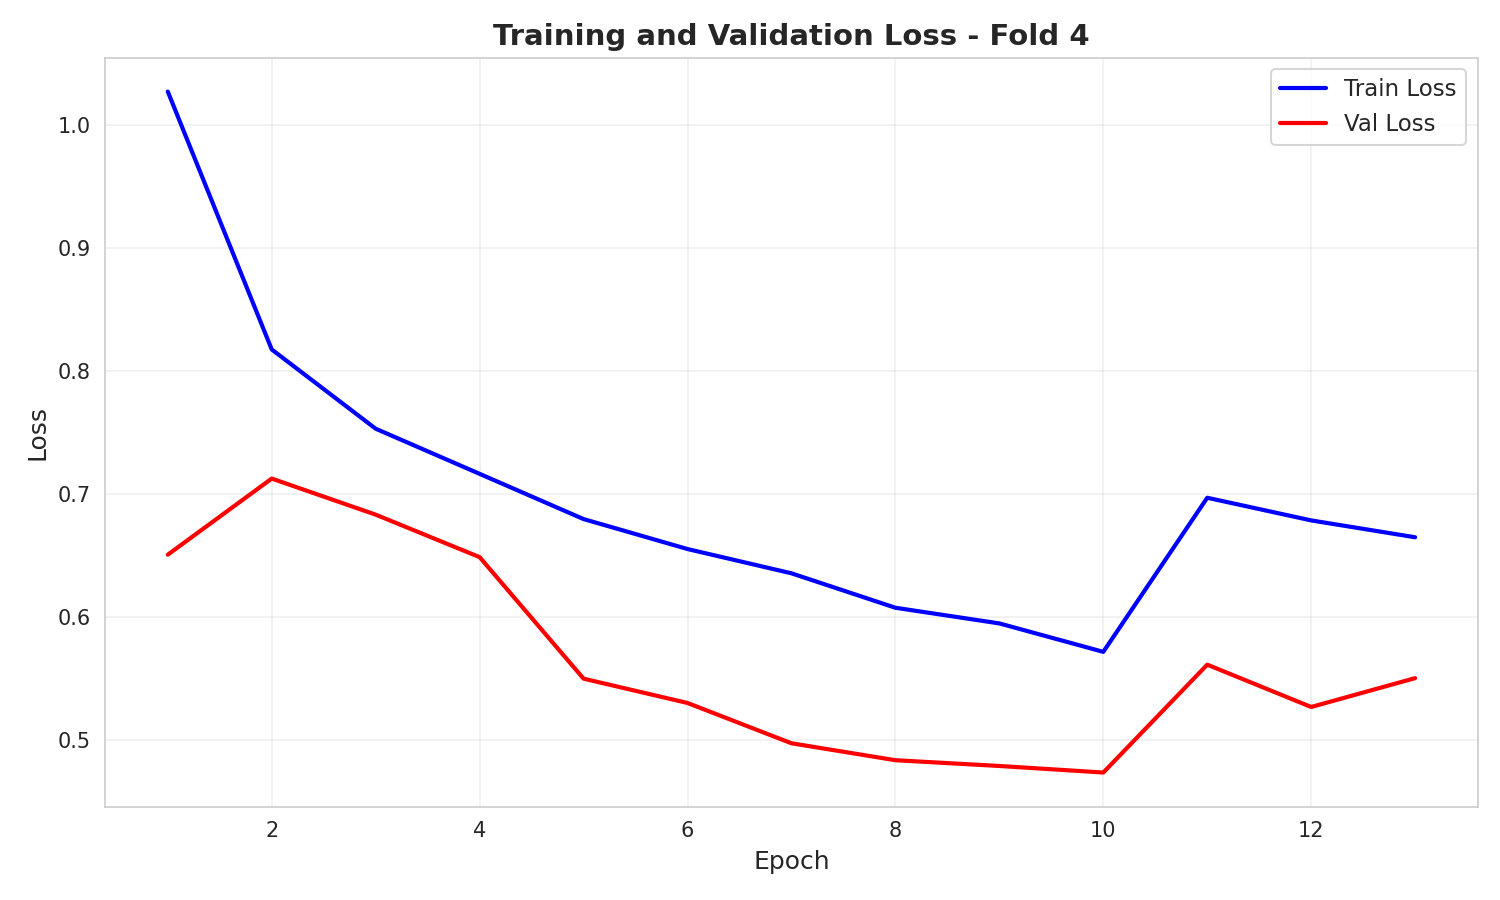
\includegraphics[width=0.45\textwidth]{figure/lampiran/lampiran_eval/resnet50_fpn_v1_amodal_adam_lr1e-04/fold4/loss_fold4.png} &
            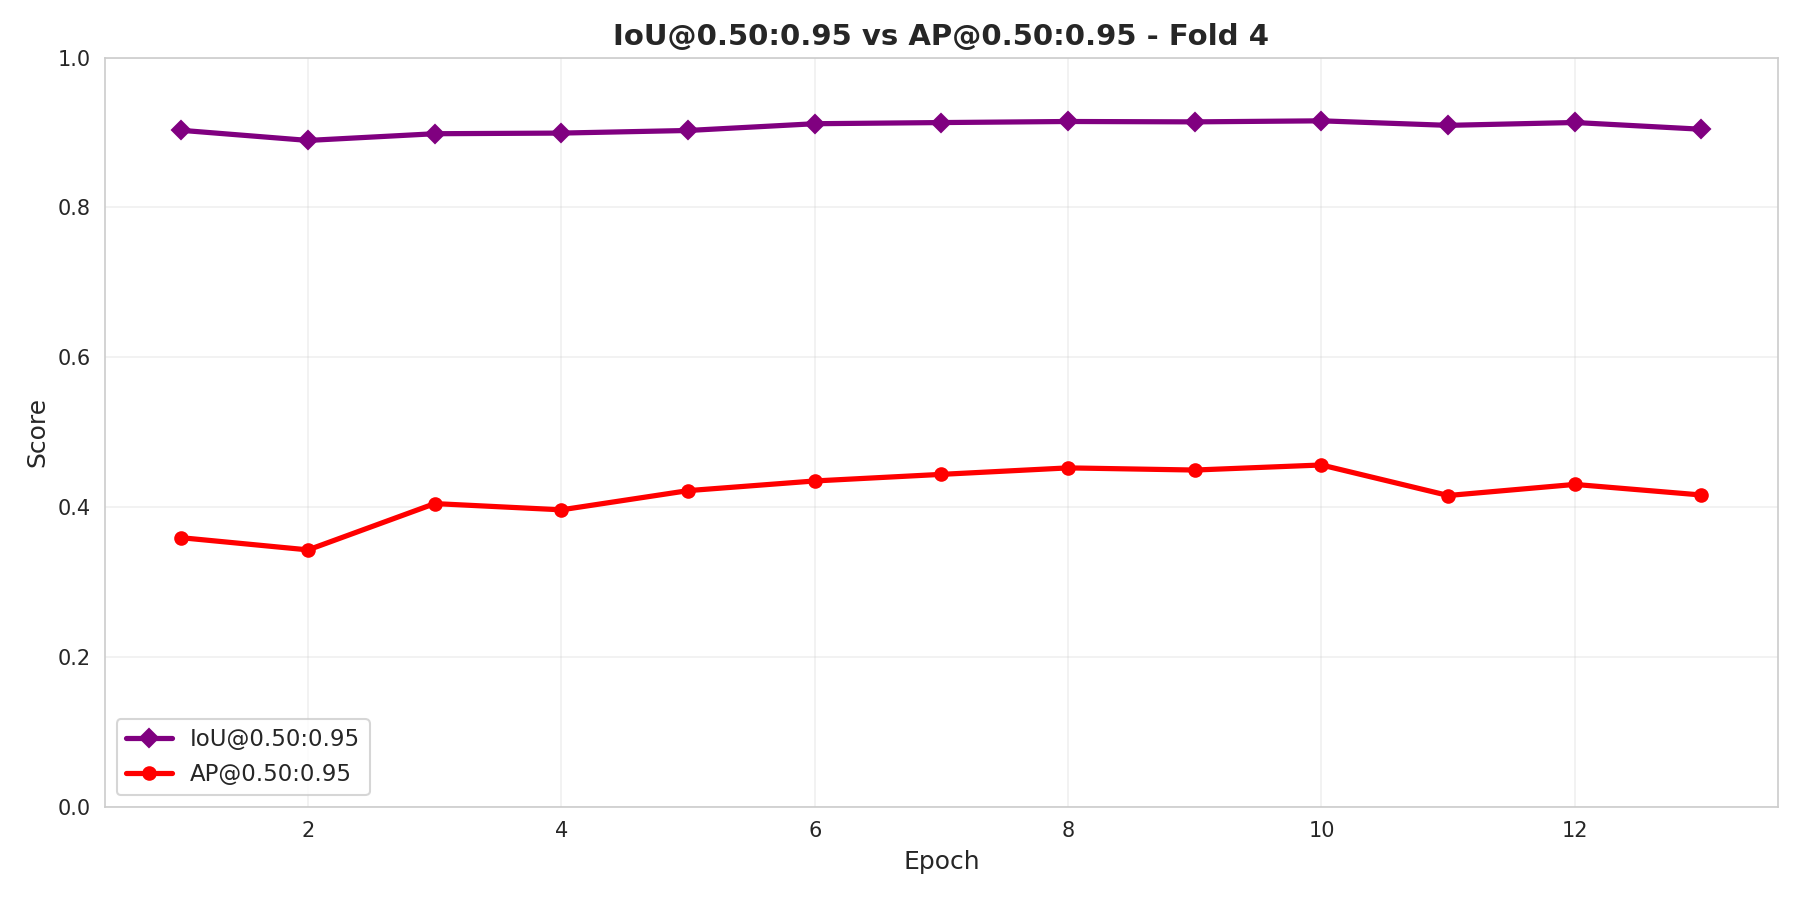
\includegraphics[width=0.45\textwidth]{figure/lampiran/lampiran_eval/resnet50_fpn_v1_amodal_adam_lr1e-04/fold4/mean_metrics_comparison_fold4.png} \\[0.5em]
            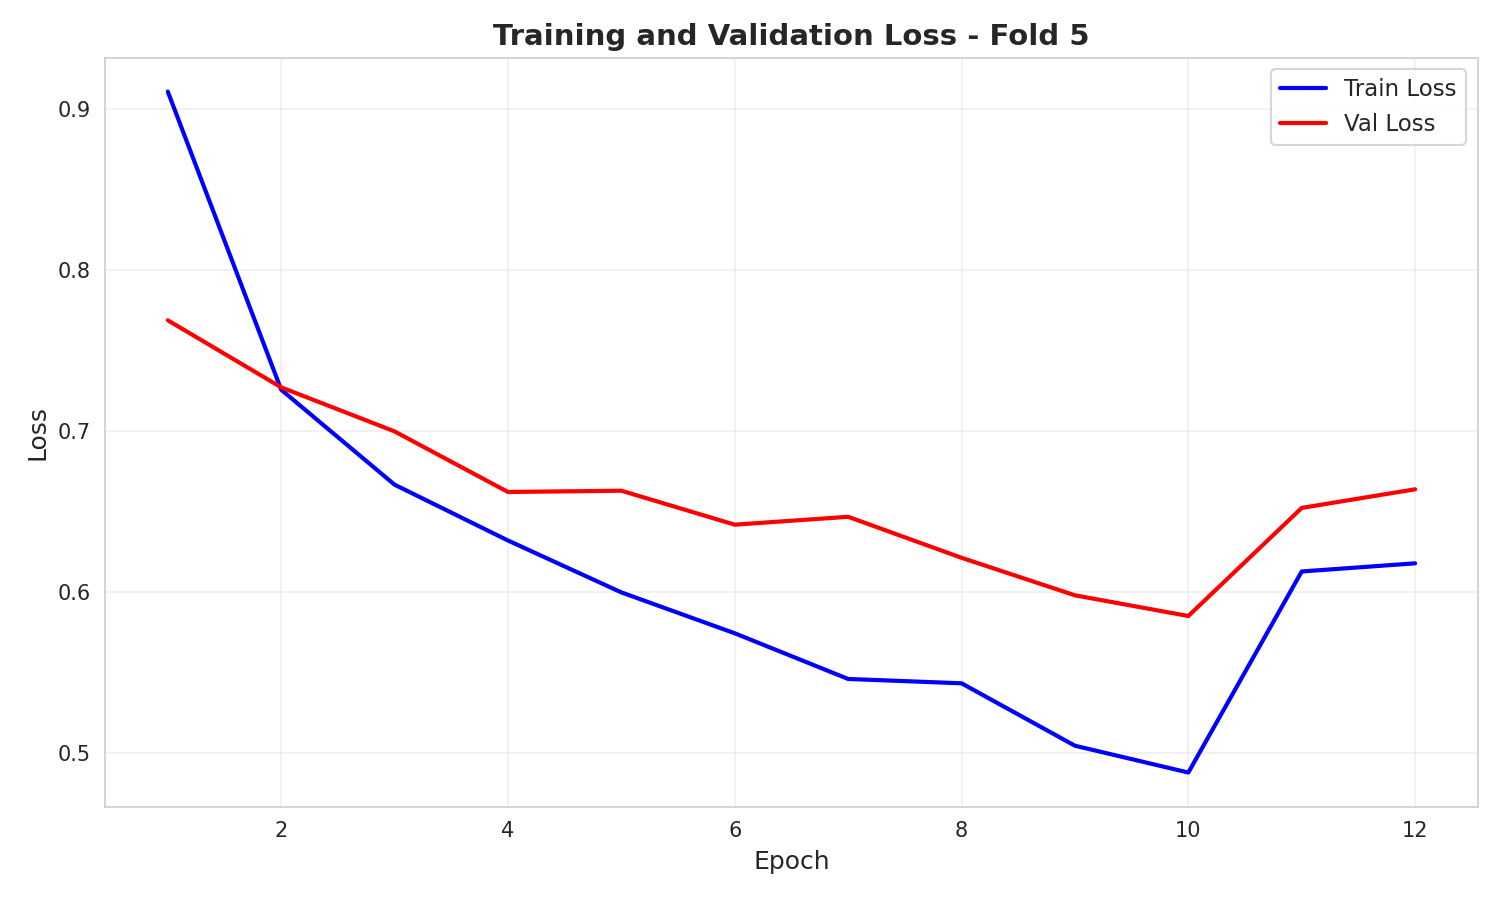
\includegraphics[width=0.45\textwidth]{figure/lampiran/lampiran_eval/resnet50_fpn_v1_amodal_adam_lr1e-04/fold5/loss_fold5.png} &
            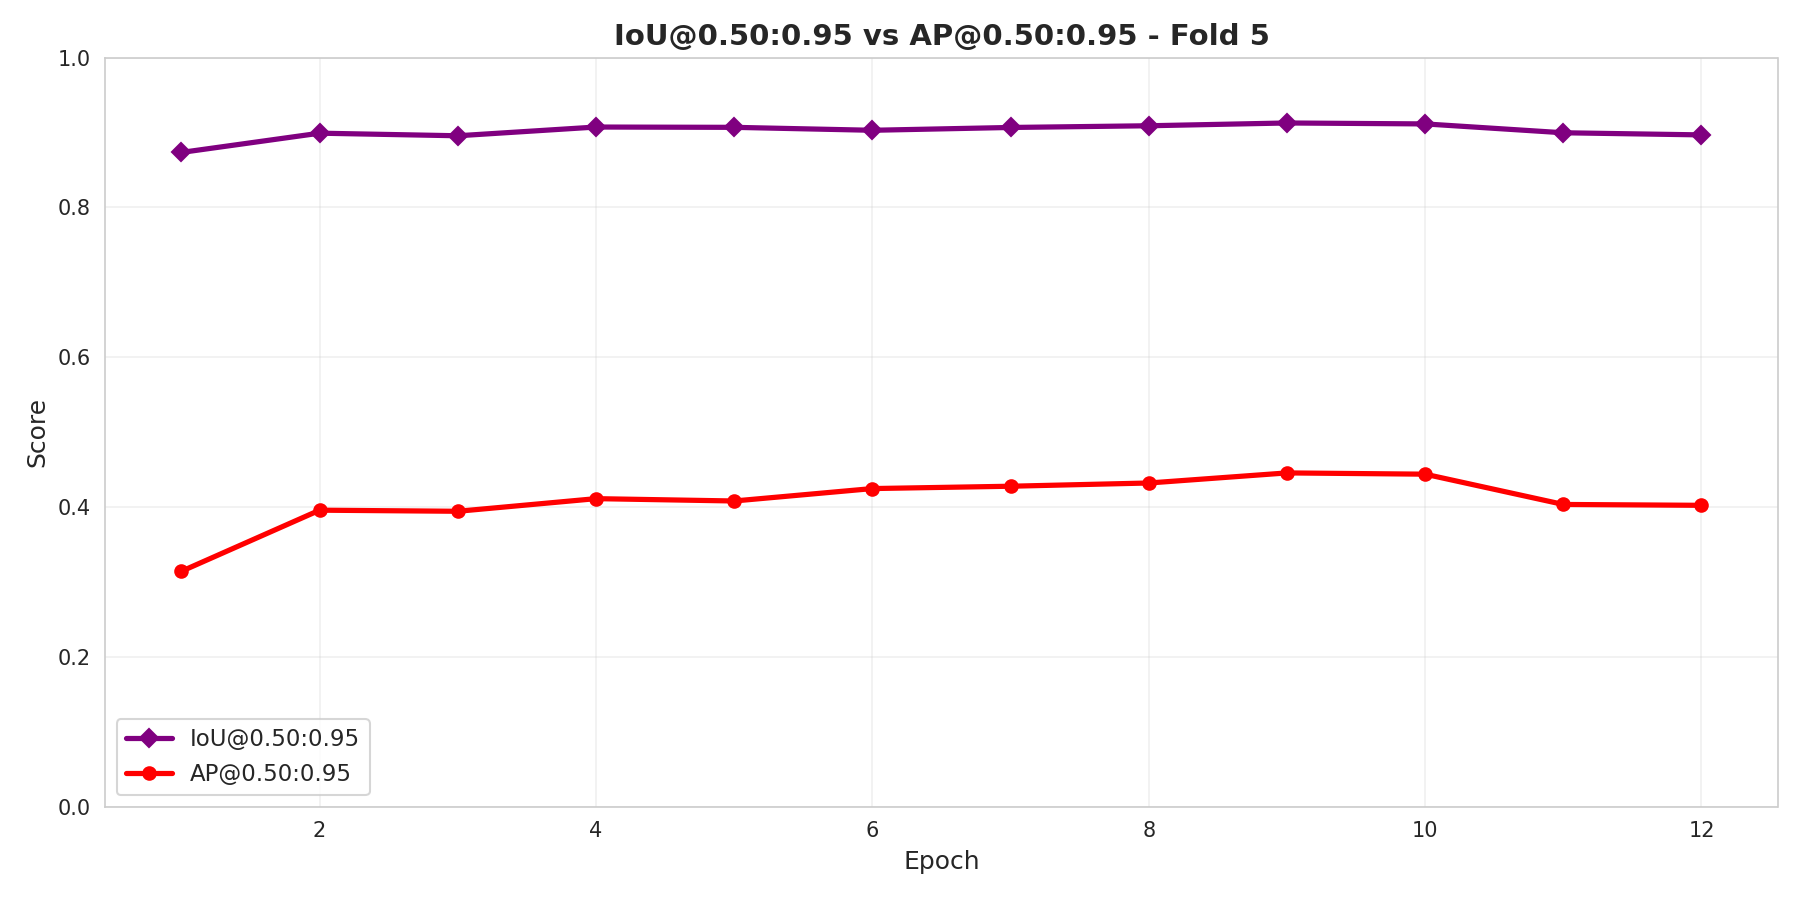
\includegraphics[width=0.45\textwidth]{figure/lampiran/lampiran_eval/resnet50_fpn_v1_amodal_adam_lr1e-04/fold5/mean_metrics_comparison_fold5.png} \\
        \end{tabular}
    \end{minipage}}
    \caption{Hasil Evaluasi Model Variasi 2 \textit{Mask} R-CNN ResNet50 FPN V1 + \textit{Amodal} + Adam}
    \label{fig:HasilEvaluasiModel2}
\end{figure}

\subsection*{Variasi 3 \textit{Mask} R-CNN ResNet50 FPN V2 + \textit{Standard} + SGD}
\begin{figure}[H]
    \centering
    \fbox{\begin{minipage}{0.95\textwidth}
        \centering
        \begin{tabular}{cc}
            
\includegraphics[width=0.45\textwidth]{figure/lampiran/lampiran_eval/resnet50_fpn_v2_standard_sgd_lr0.01/fold1/loss_fold1.png} &
            
\includegraphics[width=0.45\textwidth]{figure/lampiran/lampiran_eval/resnet50_fpn_v2_standard_sgd_lr0.01/fold1/mean_metrics_comparison_fold1.png} \\[0.5em]
            
\includegraphics[width=0.45\textwidth]{figure/lampiran/lampiran_eval/resnet50_fpn_v2_standard_sgd_lr0.01/fold2/loss_fold2.png} &
            
\includegraphics[width=0.45\textwidth]{figure/lampiran/lampiran_eval/resnet50_fpn_v2_standard_sgd_lr0.01/fold2/mean_metrics_comparison_fold2.png} \\[0.5em]
            
\includegraphics[width=0.45\textwidth]{figure/lampiran/lampiran_eval/resnet50_fpn_v2_standard_sgd_lr0.01/fold3/loss_fold3.png} &
            
\includegraphics[width=0.45\textwidth]{figure/lampiran/lampiran_eval/resnet50_fpn_v2_standard_sgd_lr0.01/fold3/mean_metrics_comparison_fold3.png} \\[0.5em]
            
\includegraphics[width=0.45\textwidth]{figure/lampiran/lampiran_eval/resnet50_fpn_v2_standard_sgd_lr0.01/fold4/loss_fold4.png} &
            
\includegraphics[width=0.45\textwidth]{figure/lampiran/lampiran_eval/resnet50_fpn_v2_standard_sgd_lr0.01/fold4/mean_metrics_comparison_fold4.png} \\[0.5em]
            
\includegraphics[width=0.45\textwidth]{figure/lampiran/lampiran_eval/resnet50_fpn_v2_standard_sgd_lr0.01/fold5/loss_fold5.png} &
            
\includegraphics[width=0.45\textwidth]{figure/lampiran/lampiran_eval/resnet50_fpn_v2_standard_sgd_lr0.01/fold5/mean_metrics_comparison_fold5.png} \\
        \end{tabular}
    \end{minipage}}
    \caption{Hasil Evaluasi Model Variasi 3 \textit{Mask} R-CNN ResNet50 FPN V2 + \textit{Standard} + SGD}
    \label{fig:HasilEvaluasiModel3}
\end{figure}

\subsection*{Variasi 4 \textit{Mask} R-CNN ResNet50 FPN V2 + \textit{Standard} + Adam}
\begin{figure}[H]
    \centering
    \fbox{\begin{minipage}{0.95\textwidth}
        \centering
        \begin{tabular}{cc}
            
\includegraphics[width=0.45\textwidth]{figure/lampiran/lampiran_eval/resnet50_fpn_v2_standard_adam_lr1e-04/fold1/loss_fold1.png} &
            
\includegraphics[width=0.45\textwidth]{figure/lampiran/lampiran_eval/resnet50_fpn_v2_standard_adam_lr1e-04/fold1/mean_metrics_comparison_fold1.png} \\[0.5em]
            
\includegraphics[width=0.45\textwidth]{figure/lampiran/lampiran_eval/resnet50_fpn_v2_standard_adam_lr1e-04/fold2/loss_fold2.png} &
            
\includegraphics[width=0.45\textwidth]{figure/lampiran/lampiran_eval/resnet50_fpn_v2_standard_adam_lr1e-04/fold2/mean_metrics_comparison_fold2.png} \\[0.5em]
            
\includegraphics[width=0.45\textwidth]{figure/lampiran/lampiran_eval/resnet50_fpn_v2_standard_adam_lr1e-04/fold3/loss_fold3.png} &
            
\includegraphics[width=0.45\textwidth]{figure/lampiran/lampiran_eval/resnet50_fpn_v2_standard_adam_lr1e-04/fold3/mean_metrics_comparison_fold3.png} \\[0.5em]
            
\includegraphics[width=0.45\textwidth]{figure/lampiran/lampiran_eval/resnet50_fpn_v2_standard_adam_lr1e-04/fold4/loss_fold4.png} &
            
\includegraphics[width=0.45\textwidth]{figure/lampiran/lampiran_eval/resnet50_fpn_v2_standard_adam_lr1e-04/fold4/mean_metrics_comparison_fold4.png} \\[0.5em]
            
\includegraphics[width=0.45\textwidth]{figure/lampiran/lampiran_eval/resnet50_fpn_v2_standard_adam_lr1e-04/fold5/loss_fold5.png} &
            
\includegraphics[width=0.45\textwidth]{figure/lampiran/lampiran_eval/resnet50_fpn_v2_standard_adam_lr1e-04/fold5/mean_metrics_comparison_fold5.png} \\
        \end{tabular}
    \end{minipage}}
    \caption{Hasil Evaluasi Model Variasi 4 \textit{Mask} R-CNN ResNet50 FPN V2 + \textit{Standard} + Adam}
    \label{fig:HasilEvaluasiModel4}
\end{figure}

\subsection*{Variasi 5 \textit{Mask} R-CNN ResNet50 FPN V2 + \textit{Amodal} + SGD}
\begin{figure}[H]
    \centering
    \fbox{\begin{minipage}{0.95\textwidth}
        \centering
        \begin{tabular}{cc}
            
\includegraphics[width=0.45\textwidth]{figure/lampiran/lampiran_eval/resnet50_fpn_v2_amodal_sgd_lr0.01/fold1/loss_fold1.png} &
            
\includegraphics[width=0.45\textwidth]{figure/lampiran/lampiran_eval/resnet50_fpn_v2_amodal_sgd_lr0.01/fold1/mean_metrics_comparison_fold1.png} \\[0.5em]
            
\includegraphics[width=0.45\textwidth]{figure/lampiran/lampiran_eval/resnet50_fpn_v2_amodal_sgd_lr0.01/fold2/loss_fold2.png} &
            
\includegraphics[width=0.45\textwidth]{figure/lampiran/lampiran_eval/resnet50_fpn_v2_amodal_sgd_lr0.01/fold2/mean_metrics_comparison_fold2.png} \\[0.5em]
            
\includegraphics[width=0.45\textwidth]{figure/lampiran/lampiran_eval/resnet50_fpn_v2_amodal_sgd_lr0.01/fold3/loss_fold3.png} &
            
\includegraphics[width=0.45\textwidth]{figure/lampiran/lampiran_eval/resnet50_fpn_v2_amodal_sgd_lr0.01/fold3/mean_metrics_comparison_fold3.png} \\[0.5em]
            
\includegraphics[width=0.45\textwidth]{figure/lampiran/lampiran_eval/resnet50_fpn_v2_amodal_sgd_lr0.01/fold4/loss_fold4.png} &
            
\includegraphics[width=0.45\textwidth]{figure/lampiran/lampiran_eval/resnet50_fpn_v2_amodal_sgd_lr0.01/fold4/mean_metrics_comparison_fold4.png} \\[0.5em]
            
\includegraphics[width=0.45\textwidth]{figure/lampiran/lampiran_eval/resnet50_fpn_v2_amodal_sgd_lr0.01/fold5/loss_fold5.png} &
            
\includegraphics[width=0.45\textwidth]{figure/lampiran/lampiran_eval/resnet50_fpn_v2_amodal_sgd_lr0.01/fold5/mean_metrics_comparison_fold5.png} \\
        \end{tabular}
    \end{minipage}}
    \caption{Hasil Evaluasi Model Variasi 5 \textit{Mask} R-CNN ResNet50 FPN V2 + \textit{Amodal} + SGD}
    \label{fig:HasilEvaluasiModel5}
\end{figure}

\subsection*{Variasi 6 \textit{Mask} R-CNN ResNet50 FPN V2 + \textit{Amodal} + Adam}
\begin{figure}[H]
    \centering
    \fbox{\begin{minipage}{0.95\textwidth}
        \centering
        \begin{tabular}{cc}
            
\includegraphics[width=0.45\textwidth]{figure/lampiran/lampiran_eval/resnet50_fpn_v2_amodal_adam_lr1e-04/fold1/loss_fold1.png} &
            
\includegraphics[width=0.45\textwidth]{figure/lampiran/lampiran_eval/resnet50_fpn_v2_amodal_adam_lr1e-04/fold1/mean_metrics_comparison_fold1.png} \\[0.5em]
            
\includegraphics[width=0.45\textwidth]{figure/lampiran/lampiran_eval/resnet50_fpn_v2_amodal_adam_lr1e-04/fold2/loss_fold2.png} &
            
\includegraphics[width=0.45\textwidth]{figure/lampiran/lampiran_eval/resnet50_fpn_v2_amodal_adam_lr1e-04/fold2/mean_metrics_comparison_fold2.png} \\[0.5em]
            
\includegraphics[width=0.45\textwidth]{figure/lampiran/lampiran_eval/resnet50_fpn_v2_amodal_adam_lr1e-04/fold3/loss_fold3.png} &
            
\includegraphics[width=0.45\textwidth]{figure/lampiran/lampiran_eval/resnet50_fpn_v2_amodal_adam_lr1e-04/fold3/mean_metrics_comparison_fold3.png} \\[0.5em]
            
\includegraphics[width=0.45\textwidth]{figure/lampiran/lampiran_eval/resnet50_fpn_v2_amodal_adam_lr1e-04/fold4/loss_fold4.png} &
            
\includegraphics[width=0.45\textwidth]{figure/lampiran/lampiran_eval/resnet50_fpn_v2_amodal_adam_lr1e-04/fold4/mean_metrics_comparison_fold4.png} \\[0.5em]
            
\includegraphics[width=0.45\textwidth]{figure/lampiran/lampiran_eval/resnet50_fpn_v2_amodal_adam_lr1e-04/fold5/loss_fold5.png} &
            
\includegraphics[width=0.45\textwidth]{figure/lampiran/lampiran_eval/resnet50_fpn_v2_amodal_adam_lr1e-04/fold5/mean_metrics_comparison_fold5.png} \\
        \end{tabular}
    \end{minipage}}
    \caption{Hasil Evaluasi Model Variasi 6 \textit{Mask} R-CNN ResNet50 FPN V2 + \textit{Amodal} + Adam}
    \label{fig:HasilEvaluasiModel6}
\end{figure}

\subsection*{Variasi 7 \textit{Mask} R-CNN ResNet50 FPN V2 + \textit{Standard} + SGD}
\begin{figure}[H]
    \centering
    \fbox{\begin{minipage}{0.95\textwidth}
        \centering
        \begin{tabular}{cc}
            
\includegraphics[width=0.45\textwidth]{figure/lampiran/lampiran_eval/resnet50_fpn_v2_standard_sgd_lr0.01/fold1/loss_fold1.png} &
            
\includegraphics[width=0.45\textwidth]{figure/lampiran/lampiran_eval/resnet50_fpn_v2_standard_sgd_lr0.01/fold1/mean_metrics_comparison_fold1.png} \\[0.5em]
            
\includegraphics[width=0.45\textwidth]{figure/lampiran/lampiran_eval/resnet50_fpn_v2_standard_sgd_lr0.01/fold2/loss_fold2.png} &
            
\includegraphics[width=0.45\textwidth]{figure/lampiran/lampiran_eval/resnet50_fpn_v2_standard_sgd_lr0.01/fold2/mean_metrics_comparison_fold2.png} \\[0.5em]
            
\includegraphics[width=0.45\textwidth]{figure/lampiran/lampiran_eval/resnet50_fpn_v2_standard_sgd_lr0.01/fold3/loss_fold3.png} &
            
\includegraphics[width=0.45\textwidth]{figure/lampiran/lampiran_eval/resnet50_fpn_v2_standard_sgd_lr0.01/fold3/mean_metrics_comparison_fold3.png} \\[0.5em]
            
\includegraphics[width=0.45\textwidth]{figure/lampiran/lampiran_eval/resnet50_fpn_v2_standard_sgd_lr0.01/fold4/loss_fold4.png} &
            
\includegraphics[width=0.45\textwidth]{figure/lampiran/lampiran_eval/resnet50_fpn_v2_standard_sgd_lr0.01/fold4/mean_metrics_comparison_fold4.png} \\[0.5em]
            
\includegraphics[width=0.45\textwidth]{figure/lampiran/lampiran_eval/resnet50_fpn_v2_standard_sgd_lr0.01/fold5/loss_fold5.png} &
            
\includegraphics[width=0.45\textwidth]{figure/lampiran/lampiran_eval/resnet50_fpn_v2_standard_sgd_lr0.01/fold5/mean_metrics_comparison_fold5.png} \\
        \end{tabular}
    \end{minipage}}
    \caption{Hasil Evaluasi Model Variasi 7 \textit{Mask} R-CNN ResNet50 FPN V2 + \textit{Standard} + SGD}
    \label{fig:HasilEvaluasiModel7}
\end{figure}

\subsection*{Variasi 8 \textit{Mask} R-CNN ResNet50 FPN V2 + \textit{Standard} + Adam}
\begin{figure}[H]
    \centering
    \fbox{\begin{minipage}{0.95\textwidth}
        \centering
        \begin{tabular}{cc}
            
\includegraphics[width=0.45\textwidth]{figure/lampiran/lampiran_eval/resnet50_fpn_v2_standard_adam_lr1e-04/fold1/loss_fold1.png} &
            
\includegraphics[width=0.45\textwidth]{figure/lampiran/lampiran_eval/resnet50_fpn_v2_standard_adam_lr1e-04/fold1/mean_metrics_comparison_fold1.png} \\[0.5em]
            
\includegraphics[width=0.45\textwidth]{figure/lampiran/lampiran_eval/resnet50_fpn_v2_standard_adam_lr1e-04/fold2/loss_fold2.png} &
            
\includegraphics[width=0.45\textwidth]{figure/lampiran/lampiran_eval/resnet50_fpn_v2_standard_adam_lr1e-04/fold2/mean_metrics_comparison_fold2.png} \\[0.5em]
            
\includegraphics[width=0.45\textwidth]{figure/lampiran/lampiran_eval/resnet50_fpn_v2_standard_adam_lr1e-04/fold3/loss_fold3.png} &
            
\includegraphics[width=0.45\textwidth]{figure/lampiran/lampiran_eval/resnet50_fpn_v2_standard_adam_lr1e-04/fold3/mean_metrics_comparison_fold3.png} \\[0.5em]
            
\includegraphics[width=0.45\textwidth]{figure/lampiran/lampiran_eval/resnet50_fpn_v2_standard_adam_lr1e-04/fold4/loss_fold4.png} &
            
\includegraphics[width=0.45\textwidth]{figure/lampiran/lampiran_eval/resnet50_fpn_v2_standard_adam_lr1e-04/fold4/mean_metrics_comparison_fold4.png} \\[0.5em]
            
\includegraphics[width=0.45\textwidth]{figure/lampiran/lampiran_eval/resnet50_fpn_v2_standard_adam_lr1e-04/fold5/loss_fold5.png} &
            
\includegraphics[width=0.45\textwidth]{figure/lampiran/lampiran_eval/resnet50_fpn_v2_standard_adam_lr1e-04/fold5/mean_metrics_comparison_fold5.png} \\
        \end{tabular}
    \end{minipage}}
    \caption{Hasil Evaluasi Model Variasi 8 \textit{Mask} R-CNN ResNet50 FPN V2 + \textit{Standard} + Adam}
    \label{fig:HasilEvaluasiModel8}
\end{figure}